\documentclass[en]{aghdpl}  % praca w języku angielskim
\usepackage[utf8]{inputenc}
\usepackage{courier}

\lstloadlanguages{TeX}

%---------------------------------------------------------------------------

\author{Dariusz Chrząścik \\
  Radosław Morytko
}


\shortauthor{D. Chrząścik, R. Morytko}

\titlePL{Adaptowalne środowisko obliczeniowe skalujące aplikacje użytkowników}
\titleEN{Self-adaptive cloud computing platform for scaling users' applications}


\supervisorPL{dr inż. Marcin Jarząb}
\supervisorEN{Marcin Jarząb}

\date{2013}

\departmentPL{Katedra Informatyki}
\departmentEN{Department of Computer Science}

\facultyPL{Wydział Informatyki, Elektroniki i Telekomunikacji}
\facultyEN{Faculty of Computer Science, Electronics and Telecommunications}

\acknowledgements{I would love to express my best wishes ..}


\setlength{\cftsecnumwidth}{10mm}

%---------------------------------------------------------------------------

\begin{document}

% front pages, statements and abstract
\titlepages

\tableofcontents

\clearpage

\chapter{Introduction}

\section{Motivation}
One of the keys factors that has driven transformation of computing industry in the last years is the perception of computing utilities as a commodity\cite{BuYeVeBrBr09}, easily accessible and adjustable to specific needs. As a consequence, we observe a profusion of different services, often collectively referred as a cloud computing \cite{MeGr11}. Similarly to services known from traditional markets, customers expect them to be accessible on demand and in easy manner, while paying only for the consumed goods. Furthermore, customers are interested in a given service only when its provider is eligible to guarantee appropriate quality of service.

The particular service providers that are addressed by this thesis are the ones that supply users with an application execution platform, a model widely known as providing Platform-as-a-Service. In that case, a customer is an entity that has developed an application and is eager to deploy it on an application platform provided that it is able to fulfil his specific requirements, both in terms of quality and cost.

Having customer requirements in mind, it is crucial that a service provider is able to adapt itself to fulfil customer's contract. For example, such adaptation can be triggered by a sudden spike in resource demand and may result in provisioning additional application platforms. However, due to the problem complexity and number of concerns involved, there are different levels where adaptation is possible:
\begin{itemize}
	\item user application
	\item application platform
	\item infrastructure
\end{itemize}
What is more, the fact that single service provider is constrained by his finite amount of resources poses a risk that it may not be able to serve customer all the time. Consequently, it is expected that adaptation at a service provider level is also possible, i.e. provider can offload some traffic to a different provider, as long as it satisfies a customer.

While self-adaptive systems have a long history \cite{Mu04}, it have not been directly applied to a multi-layered problem that exists in a cloud computing environment. Especially, the research area at the last layer, which sizes across different service providers, is new. Although, architecture known as InterCloud \cite{BuRaCa10} investigates problem of cooperation and negotiation at a cloud level, it neither has been implemented nor presented in a context of self-adaptive system.

\subsection*{Business potential}
The rapid growth of interest in cloud computing in recent years resulted in huge sums of money being invested in the field. Figure \ref{chapter-fig:public-cloud-services-market-size} shows the size of the public cloud services market in 2012 and the forecast of its nearly two times growth in 2016. This data suggests that the subject is attractive for IT industry from the economic point of view. However, higher amounts of money spent on cloud services involve higher expectations of theirs quality from customers. Although the most significant players in cloud computing have been in the field for quite a long time, it is still possible to outline some deficiencies their products have. Additionally, lack of common standards hinder cooperation among different cloud providers. For example it is nearly impossible to create an autoscaling cloud federation with Amazon Web Services (current leader in providing cloud services\cite{GartnerMagicQuadrantSep2013}) and another provider. Amazon EC2, when compared to other companies especially in terms of autoscaling capabilities, really shines. OpenShift, RedHat PaaS solution, ensures application scaling but with very limited possibilities of customisation of the process -- the user can only choose if their application should scale and the whole algorithm is solely based on the number of concurrent requests to the application. Users of Heroku, another PaaS solution, have no automation tool that would control the number of instances (\emph{dynos} in Heroku nomenclature) their application is running on -- they can change it manually.

The proposed solution in this dissertation tries to deal with the aforementioned providers problems by outlining an example architecture that enables seamless cooperation among cloud providers and provides auto-scaling capabilities.

\begin{figure}[!ht]
  \begin{center}
    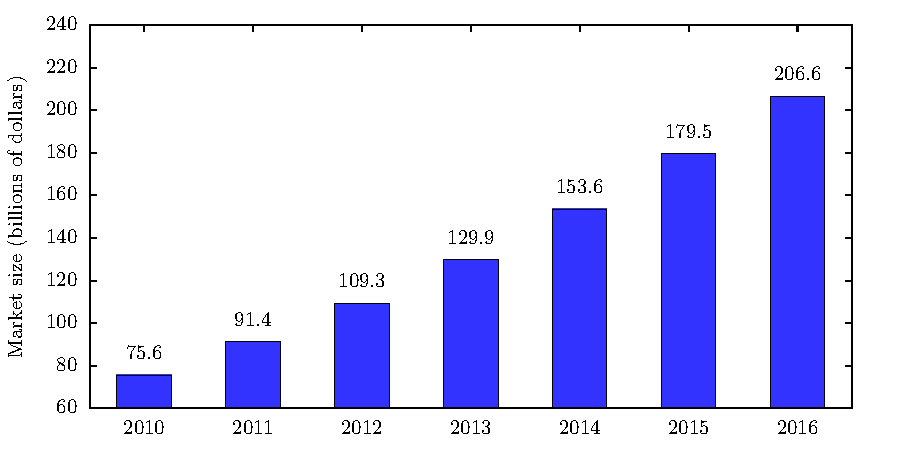
\includegraphics{chapter-introduction/public-cloud-services-market-size}
  \end{center}
  \caption{Public Cloud Services Market Size, 2010-2016 (forecast). Source: \textit{Gartner, 08/2012}}
  \label{chapter-fig:public-cloud-services-market-size}
\end{figure}

\section{Contributions}
The main contributions of this dissertation are as follows:
\begin{itemize}
  \item A proposal of an architecture of federated cloud computing environment, which is based on and can be viewed as a simplified version of \emph{InterCloud}
  \item The notion of considering each service model as an autonomic system
  \item The implementation of the proposed architecture using OpenNebula technology stack
  \item The evaluation of implemented proof-of-concept
\end{itemize}

\section{Impact}
We hope that the concept of representing each level of an autoscaling subsystem as an autonomic one can be thought-provoking for cloud computing scientists.  What is more, we believe that our successful attempt to implement a simplified variant of an InterCloud architecture will cause its gain in interest and popularity. 
Finally, we consider the ideas contained in this work be beneficial to the OpenNebula ecosystem as they provide insights into the ways Quality of Service can be ensured:
\begin{itemize}
  \item implementing autoscaling capabilities
  \item designing \emph{cloud infrastructure} in accordance with InterCloud architecture
\end{itemize}

\section{Thesis structure}


\chapter{Problem domain}
\chapterintro{This chapter details mechanisms and practises that ensures a Quality-of-Service level is met by means of a self-adaptive system that scales across multiple service providers.}

\section{Self-adaptive system}

\subsection{Introduction}
Guaranteeing Quality-of-Service can be seen as continuous monitoring and reacting to undesirable conditions when necessary. In fact, this process is an IT procedure performed by system administrator. Figure \ref{fig:it-process} illustrates an example of such procedure. While system administrator can be directly responsible for manually performing steps depicted in figure \ref{fig:it-process}, it is much more favourable to automatize this process leading to a self-manageable system. Not only does it lead to efficiency of an IT process but also to its effectiveness \cite{IBM06}. It is achieved through:
\begin{itemize}
  \item \emph{rapid process initiation} - components auto-initiate actions based on information derived from a system
  \item \emph{reduced time and skill requirements} - automatization of IT processes makes them easier and less troublesome what is especially important for skill-intensive, error-prone and long lasting tasks
\end{itemize}

\begin{figure}[!ht]
  \begin{center}
    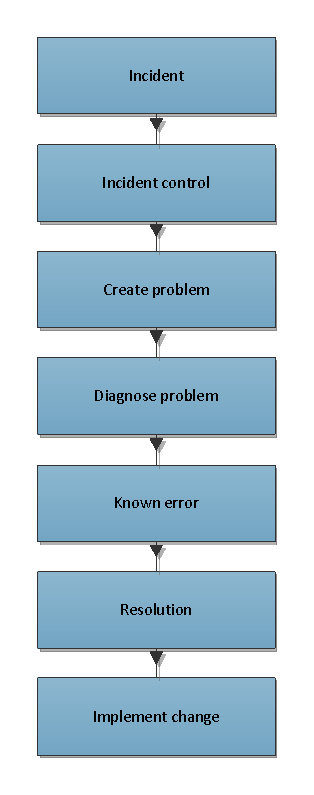
\includegraphics{chapter-adaptivity/it-process}
  \end{center}
  \caption{Exemplary IT process}
  \label{fig:it-process}
\end{figure}


In the heart of the every self-adaptive systems, according to \cite{brun2009engineering}, lies a feedback loop, concept that originates from a control engineering. As paper's authors advocate:
\begin{quote}
Feedback loops provide the generic mechanism for self-adaptation. Positive feedback occurs when an initial change in a system is reinforced, which leads toward an amplification of the change. In contrast, negative feedback triggers a response that counteracts a perturbation. 
\end{quote}

What control loop is made of is:
\begin{inparaenum}[1)]
 \item collection of data
 \item data analysis
 \item making a decisions
 \item enforcing actions
\end{inparaenum}
Figure \ref{fig:feedback-loop} depicts a generic feedback loop, giving context associated with each phase. Successive sections details aforementioned phases.

\begin{figure}[!ht]
  \begin{center}
    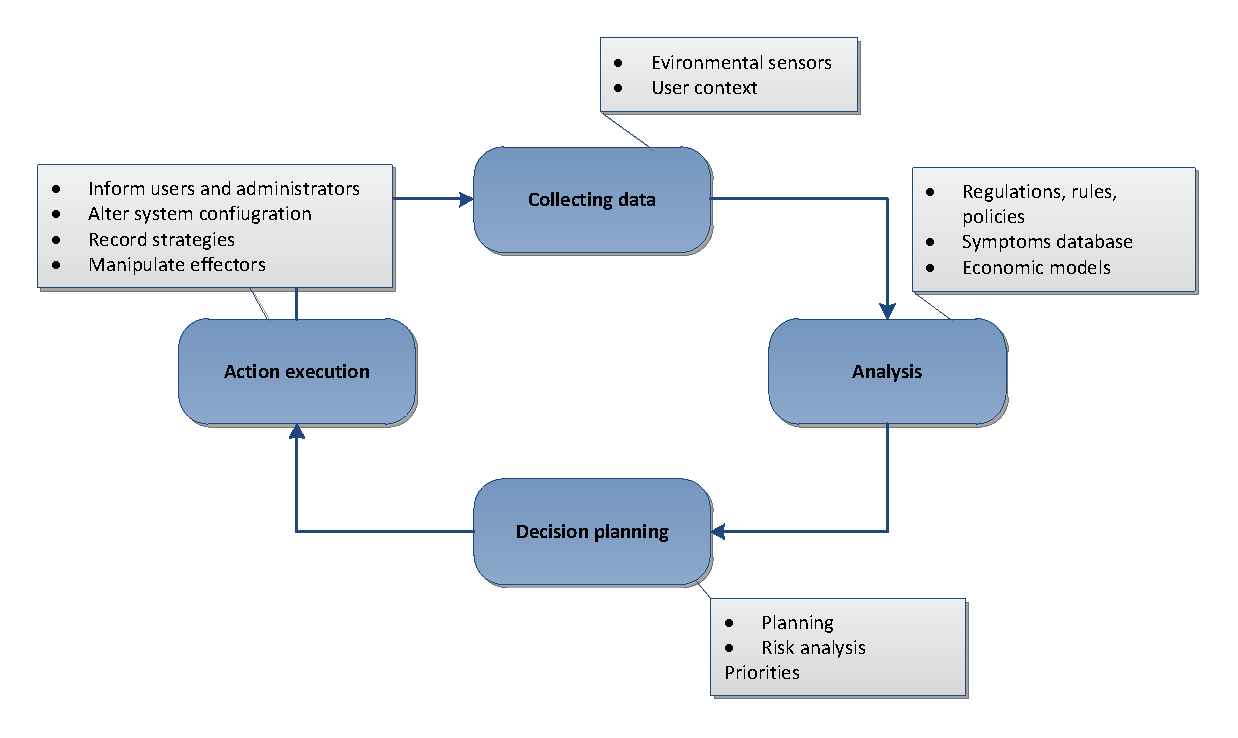
\includegraphics[width=\textwidth]{chapter-adaptivity/feedback-loop}
  \end{center}
  \caption{Feedback loop \cite{brun2009engineering}}
  \label{fig:feedback-loop}
\end{figure}

\subsection{Collecting data}
During this phase, relevant data is collected from sensors. After that, data can be aggregated, filtered or stored to provide a reference point during future feedback loop evaluation. During this phase, there are a few concerns that should be investigated \cite{brun2009engineering}:
\begin{itemize}
 \item sample rate
 \item probe reliability
 \item data format
\end{itemize}

Almost any cloud platform providers incorporates into its solution monitoring component, responsible for data collection. Mechanisms used vary from providers to provider and may involve mixture of protocols and standards. For example, Carina \cite{Carina} uses OpenNebula IM and VMM drivers relaying on a plaintext data, transferred through a SSH connection.

\subsection{Analysis}
Analysis part applies mathematical models to reason about data gathered during previous phase. It can leverage variety of approaches and be driven by a customer-defined policies.

As \cite{brun2009engineering} specifies, it is important to take into account following concerns during analysis phase:
\begin{itemize}
 \item applying historical data and existing patterns to current situation
 \item archiving data
 \item applying adequate model to current situation
 \item model's stability
\end{itemize}

Currently, service providers employs only simplified models such as threshold model \cite{LiWoZh05}, that defines a valid range for a given metric. In cases when it is violated (i.e. value is either smaller than minimal or bigger than maximal acceptable) corresponding resource is properly adjusted - figure \ref{fig:threshold-model} illustrates that idea.

\begin{figure}[!ht]
  \begin{center}
    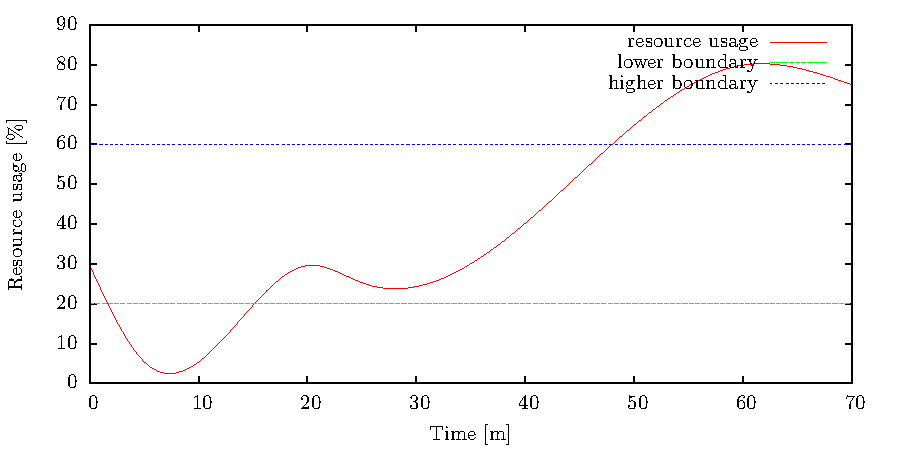
\includegraphics{chapter-adaptivity/threshold-model}
  \end{center}
  \caption{Threshold model}
  \label{fig:threshold-model}
\end{figure}

Threshold model, while trivial in its form, has been proved useful in a real-world scenarios as it is in case of AWS, OpenShift, Carina or OneCloud.

As it was already mentioned, models are often controlled by a policies that denotes a condition which, when satisfied, triggers an action, harnessing environment's disturbance. Currently, industry leaders supports \cite{AmazonAutoScaling} two kind of policies:
\begin{itemize}
 \item \textit{expression based} - allows to define how to scale application in response to changing conditions, which include factors such as memory, CPU usage, cost or some indirect, calculated metrics
 \item \textit{scheduled} - allows to scale an application in response to predictable load changes. For example, traffic increases during the weekends and decreases on working days. Hence, that predictable traffic patterns is used to scale application based on current time.
\end{itemize}

Technically, policies are expressed in a human-readable format such as JSON, XML as it is in case of AWS EC2 or custom expression used for example by Carina. Appendix \ref{app:scaling-policies} presents XML format adopted by AWS E2 Auto-Scaling.

\subsection{Decision arrangement}
Before implementing changes in an environment, decision what resources have to be tuned in order to reach a desirable state is made. Decision should be made on the basis of:
\begin{itemize}
 \item risk analysis - analysing how change effects whole environment
 \item prioritising identified problems and resources
\end{itemize}

In a case of platform-as-a-service providers, none of them explicitly specifies how a change plan is composed.

\subsection{Actions}
Finally, a change plan is implemented in a system. Actions can cover a variety of scaling and resource tuning operations. Next chapter investigates problem of scaling applications in detail.

\newpage
\section{Scaling applications}

\subsection{Introduction}

The reason why scaling application lies in our area of interest is the fact that it is widely accepted measure for improving application performance, consequently increasing offered Quality-of-Service. Enriching system with capability to scale entails avoiding additional costs that are related to coping with excessive traffic. In some cases, these costs may be caused by not handling extra traffic at all and may involve aspects such as: increased response time, processing overhead, space, memory, or money \cite{Bo00}. 

While scalability is a widely used term, it still lacks a clear and concise definition. Over the time, there were a few attempts to define it, yet not all of them were claimed as successful \cite{Hi90} \cite{DuRoWi06}. Hence, it is necessary to clarify this term before going into further discussion. Instinctively, scalability is perceived as ability of a system to accommodate an increasing number of elements or objects to process. In particular, we can point out different types of scalability that are affected by increased number of requests: \cite{Bo00}:
\begin{itemize}
	\item \textit{load scalability} - ability to work without delays and unproductive resource consumption at light, moderate, or heavy loads while making good use of available resources. Factors that may hinder load scalability include: scheduling shared resource, self-expansion, inadequate exploitation of parallelism
	\item \textit{space scalability} - memory requirements do not grow to intolerable levels as the number of items system supports increases
	\item \textit{space-time scalability} - system continues to function gracefully as the number of objects it encompasses increases by orders of magnitude
	\item \textit{structural scalability} - implementation or standards do not impede the growth of the number of objects system encompasses
\end{itemize}
Although, all of the aforementioned aspects are vital for any application, our work focuses solely on the first type of scalability. The reasoning behind this statement is that, while all of these scalability types lies in direct responsibility of an application developer, the load scalability can be additionally improved by adding additional resources to a system. This brings us to a question what kind of resources are used by an application or more appropriately in context of this dissertation: \textit{what kind of resources can we add to improve application performance?} Required resources varies from an application to an application. However, among the most common ones we can distinguish:
\begin{itemize}
	\item CPU
	\item memory
	\item storage
	\item network bandwidth
\end{itemize}

It is commonly agreed that there are two main possible ways the resource can be added:
\begin{itemize}
	\item \textit{horizontal scaling (scaling out)} - adding more nodes to a system, such as servers in a context of distributed application
	\item \textit{vertical scaling (scaling up)} - increasing capacity of a single node in a system, i.e. adding additional memory, CPU, storage, etc.
\end{itemize}

What makes scaling application particularly interesting are the benefits offered by a cloud computing, especially the illusion of a virtually infinite computing infrastructure \cite{VaRoBu11}. Making use of virtualization technologies, which often underpins cloud computing platform, allows for resource manipulation in a dynamic, on-demand manner. Although, cloud computing offers additional scaling capabilities, it increases solution complexity since they operate in different layers: server, platform, network as stated in \cite{VaRoBu11}. However, since platform containers are often represented either as virtual machines or another isolated environment (e.g. OpenShift leverages SELinux and cgroups) they are similar in nature to server scaling and supports both scaling up and out. Therefore, the remaining of this chapter is focused solely on server scaling, omitting network scaling as it lays outside of scope of this dissertation.

Having that said, common sense dictates that adding resources is only a part of the success - it should be accompanied by tuning application platform configuration. For example, adding supplementary CPUs without increasing thread pool size that handle requests makes a little sense. Similarly, in context of a Java application, we have to increase heap size, to make a good use of extra memory. While importance of application tuning cannot be underestimated, its detailed analysis lies outside of the scope of this dissertation. Figure \ref{fig:scalability-layers} presents different scalability layers and actions that can be taken at each level to improve application performance.

\begin{figure}[!ht]
  \begin{center}
    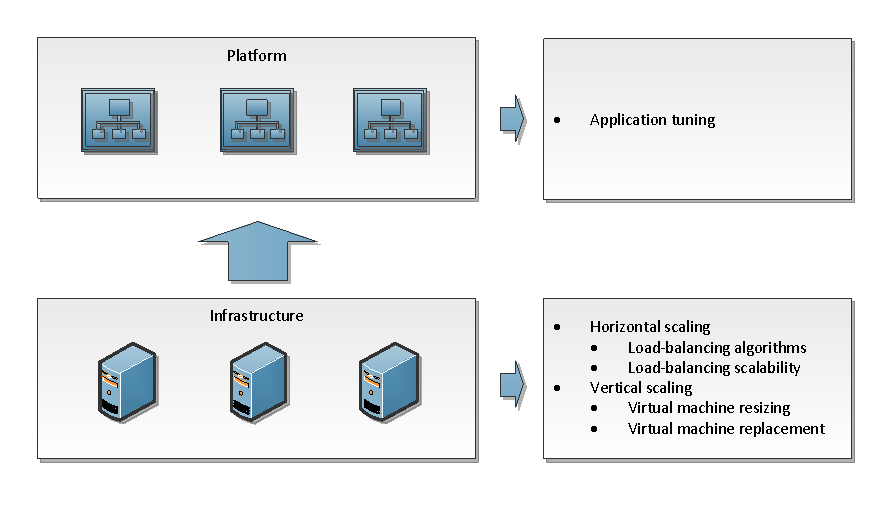
\includegraphics{chapter-scalability/scalability-layers}
  \end{center}
  \caption{Scalability layers}
  \label{fig:scalability-layers}
\end{figure}

With all that said, there is no silver bullet - not matter what underlying mechanism platform provider decides to use, the application developer is still responsible for creating an application with scaling in-mind. This statement has been already proven in 1967 by Amdahl law, which in short states that sequential component of a parallel algorithm impacts efficiency for a sufficiently large number processors \cite{Am67} as shown in Figure \ref{fig:amdahl-law}. In other words, adding supplementary resources to a poorly written application (i.e. having a lot of sequential or synchronized components) can be beneficial only to a certain degree. 

\begin{figure}[!ht]
  \begin{center}
    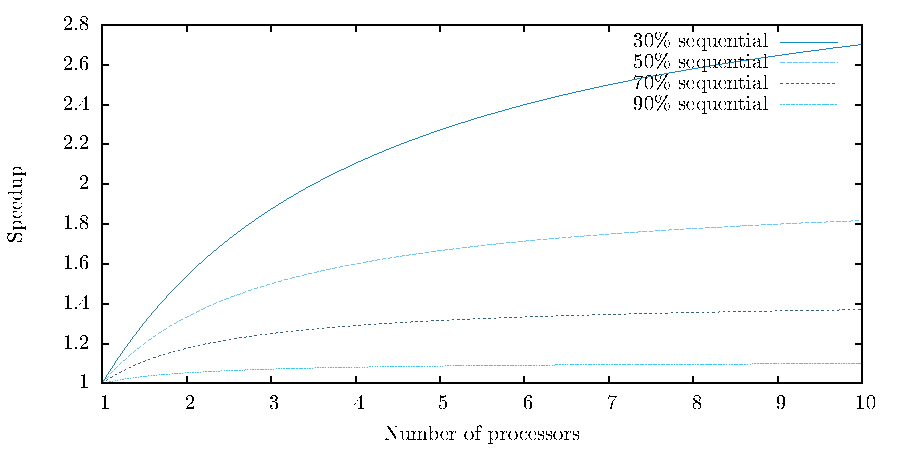
\includegraphics{chapter-scalability/amdahl-law}
  \end{center}
  \caption{Amdahl's law}
  \label{fig:amdahl-law}
\end{figure}

The rest of this chapter elaborates in detail about horizontal and vertical scaling taking into account mechanisms used in Platform-as-a-Service solutions that are available on the market.

\subsection{Horizontal scaling}
As outlined in previous section, horizontal scaling is about adding supplementary nodes to a system. As it is common to cloud computing, nodes are represented as virtual machines and this assumption is used in further discussion. Consequently, adding server comes down to cloning a new virtual machine from a template and possibly installing additional software and reconfiguring it later. While mechanism of creating new virtual machine from a template is offered literally in every IaaS platform currently available (OpenStack \cite{OpenStack}, OpenNebula \cite{OpenNebula}, CloudStack \cite{CloudStack} or Eucalyptus \cite{Eucalyptus} to name a few) and is similar in manner, the underlying hardware and virtualization mechanism determines how fast provisioning is done. 

Provisioning new server is only a first step in scaling an application, it is required to configure load balancing mechanism to make use of additional node. The two important aspects that have to be consider are: load-balancing algorithms and scalability.

\subsubsection{Load-balancing algorithms}
Generally, there are two types of load-balancers: hardware and software based. Due to the dynamic nature of system under consideration, we focus only on the latter as it offers a greater deal of flexibility. Among the most common algorithms we can distinguish \cite{HaProxyDoc}:
\begin{itemize}
 \item \textit{round-robin scheduling} - request are sent to successive nodes, according to their weights. This algorithm is fairest when the server's processing time remains equally distributed \cite{HaProxyDoc}
 \item \textit{least connection} - the server with the lowest number of connections receives the connection
 \item \textit{source routing} - source IP address is hashed, the same client IP address always reaches the same server
 \item \textit{URI hashing} - URI that designates resource is hashed and divided by the total weight of the running servers. Such hash designates which server that receives the request. In practice, this algorithm is commonly used with proxy caches and anti-virus proxies in order to maximize the cache hit rate.
 \item \textit{request counting algorithm} - load is distributed the requests among the various workers, ensuring that each gets their configured share of the number of requests
 \item \textit{weighted traffic counting algorithm} - variation of above-mentioned algorithm with a difference that it is focused on bytes rather than number of request
 \item \textit{pending request counting algorithm} - scheduler keeps track of how many requests each worker is assigned at present. A new request is automatically assigned to the worker with the lowest number of active requests
\end{itemize}

Situation gets further complicated when considering real-world web application that sends user information using cookies, what imposes requirement on load-balancer for session stickiness \cite{StBaMa11}. 

\subsubsection{Load-balancing scalability}
Although, it may seem that balancing workloads eliminates problem of a single point of failure (SPOF) among different servers, it is in fact shifted to load-balancing layer. In other words, load-balancer becomes a new SPOF. Therefore, in cases where high availability is required, multi-tiered load balancing architecture should be considered. This, however, seems not to be a case among IaaS or PaaS providers - none of them unequivocally specifies whether their provide redundancy at load-balancer level.

\subsubsection{Load-balancer comparision}

While there are many load-balancers available on the market, following are credited to be most popular:
\begin{itemize}
 \item \textbf{HAProxy} \cite{HAProxy} - load-balancer initially written by Willy Tarreau. Noticeably, it's used by OpenShift \cite{OpenShift} to distribute load among gears \cite{OpenShiftScaling}
 \item \textbf{BIG-IP Local Traffic Manager (LTM)} - solution offered by F5 \cite{F5}. Although LTM is a hardware solution, omitted in this section, it also has also its virtualized counterpart.
 \item \textbf{Apache HTTPD} \cite{ApacheHTTPD} - popular HTTP server. When enhanced with additional modules, it can behave like a proxy or load-balancer. Over the time, there were several attempts to develop such modules: mod\_jk \cite{ApacheModJk}, mod\_proxy\_balancer \cite{ApacheModProxyBalancer}, to name a few. While the former is purely AJP13 oriented, the latter supports different protocols: HTTP, FTP and AJP13. As a consequence, only mod\_proxy\_balancer was taken into account during comparision.
\end{itemize}

Table \ref{tab:load-balancer-comparison} presents they key performance features and algorithm used to schedule requests.

\begin{table}[!htbp]
\begin{tabularx}{\textwidth}[]{ X  X  X }
\specialrule{.1em}{.05em}{.05em} 

  & \textbf{Performance features} & \textbf{Scheduling algorithms} \\
\specialrule{.1em}{.05em}{.05em} 

HAProxy \cite{HAProxy} & 
-- a single-process, event-driven model reduces the cost of context switch and the memory usage
 
-- O(1) event checker
 
-- single-buffering without copying data between reads and writes
 
-- zero-copy forwarding
 
-- optimized HTTP header analysis: headers are parsed an interpreted on the fly
 
&
-- round-robin scheduling

-- least connection

-- source routing

-- URI hashing
\\ \hline

BIG-IP Local Traffic Manager \cite{LTM} &
-- managing at application services level rather than at individual devices and objects

-- scripting language that allows administrator to intercept, inspect, transform, and direct application traffic

-- built-in firewall protection, application security, and access control

-- real-time protocol and traffic management decisions
& 

\\ \hline

Apache HTTPD \cite{ApacheHTTPD} & 
-- support for session stickiness by using cookies and URL encoding. This approach \cite{ApacheModProxyBalancer} avoids unequal load distribution if clients are hidden behind proxies and stickyness errors when a client uses a dynamic IP address that changes during a session
& 
-- request counting algorithm

-- weighted traffic counting algorithm

-- pending request counting algorithm
\\ \hline

Zeus Load Balancer \cite{Zeus} & 

-- Layer-7 traffic management

-- HTTP content compression

-- connection concurrency control

-- server health monitoring

& 
-- content-aware algorithms
\\ \hline

Zeus Global Load Balancer \cite{ZeusGlobal} & 

-- service health monitoring

-- active - passive failover

-- balancing is based on observed performance

& 
-- geographic proximity

-- adaptive load balancing (based on proximity and load)

\\ \hline

\end{tabularx}

\caption{Comparison of load balancers}
\label{tab:load-balancer-comparison}

\end{table}

\newpage
\subsection{Vertical scaling}
Essentially, vertical scaling is concentrated upon increasing capacity of single node. Again, when considering technical advancements that comes with cloud computing and virtualization, we can differ two categories of scaling: virtual machine resizing and virtual machines replacement. This distinction is dictated by limitation hypervisors - not all of them are able to resize virtual machine without shutting it down.

\subsubsection{Virtual machine resizing}


\begin{table}[!htbp]
\begin{tabularx}{\textwidth}{ l  X  X  X }
\specialrule{.1em}{.05em}{.05em} 
 & \textbf{Memory} & \textbf{CPU} & \textbf{Disk} \\
\specialrule{.1em}{.05em}{.05em} 

KVM 1.2.0 &
  & 
-- dynamic pinning CPU to a specific virtual machine (depending on underlying hardware)
& 
-- adding a disk to a LVM group

\\ \hline
Xen 4.3 & 
-- changing the amount of host physical memory assigned to virtual machine without rebooting it

-- start additional virtual machines on a host whose physical memory is currently full, by automatically reducing the memory allocations of existing virtual machines in order to make space
&
-- dynamic pinning CPU to a specific virtual machine (depending on underlying hardware)
&
-- dynamic block attaching, adding a disk to a LVM group

\\ \hline
VMware ESX 5.1 &
-- hot-plugging memory, ex. using VMware vSphere
&
-- hot-plugging CPU, ex. using VMware vSphere
&
-- adding additional disks to existing virtual machine

\\ \hline
OpenVZ (kernel: 042) &
-- configurable via user beancounters
&
-- configurable via user beancounters 
& 
-- configurable via user beancounters
\\ \hline
\end{tabularx}
\caption{Comparison of hypervisors resizing capabilities}
\label{tab:hypervisors-resizing}
\end{table}


\subsubsection{Virtual machine replacement}
As it was highlighted in previous section, reasoning behind virtual machine replacement is that, in case when dynamic resizing is not possible, a new virtual machine with a desired configuration can be provisioned and replace the old one. Since this is a basic operation, all above-mentioned hypervisors supports this scenario as long as required resources are available. 


\chapter{Interoperability of clouds}

\chapterintro{This chapter introduces the notion of a hybrid cloud and explains its role in IT industry. On top of this deployment model, the concept of InterCloud is presented and elaborated with the emphasis on its application in ensuring scalability of users' services.}

\section{Introduction}
From the perspective of a user of PaaS services it is vital that they are able to deploy seamlessly their applications using libraries, tools and services supported by the cloud provider\cite{MeGr11}. Judging by such factors as the popularity of Heroku -- currently one of the most popular PaaS providers which does not offer more advanced features which would enable management of the infrastructure underpinning the deployment platform, the fact that Microsoft added auto-scaling to its Azure platform as late as in June 2013, it is perfectly possible most PaaS users are satisfied with the current offers of their providers and do need another, more sophisticated functionalities. However, there are more complex applications and systems whose requirements regarding technology stack, availability and scalability are considerably more demanding. For such services there ought to be designed slightly specialized features that would require cooperation among different cloud providers.

\section{Hybrid cloud}
One can imagine scenarios in which customers of cloud services know their applications are vulnerable to sudden variations in demand and their responsiveness must be kept at the same level all the time. In such cases, they want them to scale dynamically according to current load or other predefined or manually specified metrics. What is more, in order to ensure high availability of their services, customers do not want to confine themselves to only one provider -- in the best scenario they want their applications (or their logical parts, such as persistence layer) to be spanned across different providers and be able to cooperate with one another at the same time. Additionally, due to privacy concerns of the sensible data, companies are reluctant to put it in the public cloud storage. All these factors lead to the concept of a \emph{hybrid cloud}\cite{MeGr11} -- the case in which the cloud is a composition of two or more distinct infrastructures which are unique entities, but there are technological means that make it possible to port data and applications among them.

\subsection{Deployment models}
The informal introduction to the concept of a \emph{hybrid cloud} in the previous section requires a strict definition, but it is virtually impossible without defining other deployment models:
\begin{itemize}
  \item Private Cloud -- The provisioned cloud infrastructure is used exclusively by a single organization (that may consist of many business units) and may be owned, managed and operated by the organization or a third party.
  \item Public Cloud -- The provisioned cloud infrastructure is used by general public and may be owned, managed and operated by a business, academic or government organization or some combination of them. It exists on the premises of the cloud provider.
  \item Community Cloud -- The cloud infrastructure is provisioned for exclusive use by a specific community of consumers from organizations that have shared concerns (e.g., mission, security requirements, policy , and compliance considerations). It may be owned, managed , and operated by one or more of the organizations in the community, a third party, or some combination of them, and it may exist on or off premises. 
\end{itemize}
Having defined those models, we can see that \emph{hybrid cloud} can be placed among them and be defined as a model in which the provisioned infrastructure is a composition of two or more other infrastructures - \emph{private},\emph{community} or \emph{public}.

\subsection{Current usage and trends}
\subsubsection*{Cloud -- clients' view}
Before digging into the details of current usage and popularity of the hybrid model, it is worth discussing the general attitude of clients towards cloud computing. As the recent survey \cite{NBSurvey13} shows, the major factor that prevents companies from adopting cloud solutions is their concern over security -- in 2012 as much as 52\% responders considered it as a main concern with the regard to cloud in general. However, the tendency is that more and more enterprises do not find it a major issue as in 2012 the number declined to 46\%.
Complexity related to the management of cloud components, Vendor lock-in, interoperability and reliability were among the most frequent obstacles to adoption in 2013 for they constituted 46\%, 35\%, 27\% and 22.3\% of responders' votes respectively. Total results are shown in the figure \ref{fig:cloud-computing-adoption-obstacles-2013}.
\begin{figure}[!ht]
  \begin{center}
    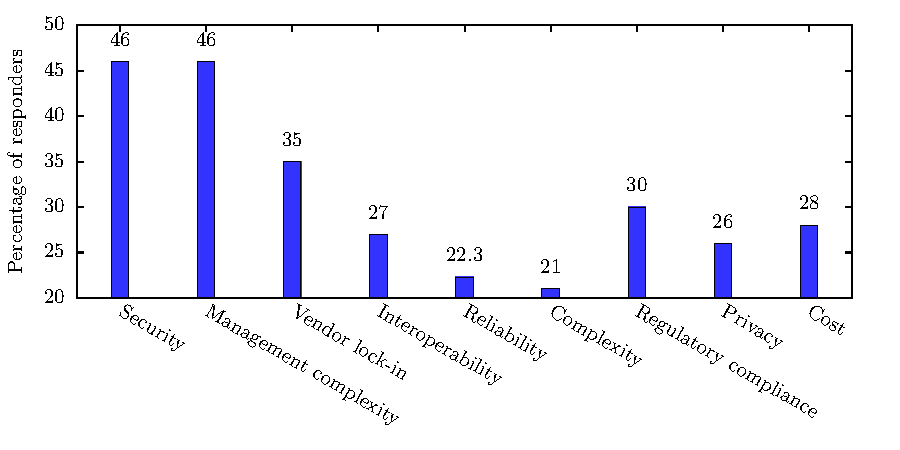
\includegraphics{chapter-interoperability/cloud-computing-adoption-obstacles-2013}
  \end{center}
  \caption{Major obstacles to cloud adoption in 2013 according to \cite{NBSurvey13}}
  \label{fig:cloud-computing-adoption-obstacles-2013}
\end{figure}

The same survey shows that the cloud adoption growth rate is high -- 75 percent of responders stated usage of some sort of a cloud platform. This means 8 percent growth when compared to the results obtained in 2012. The expectations for the total worldwide addressable market for cloud computing are to reach \$158.8B by 2014 -- an increase of 126.5 percent from 2011.

\subsubsection*{View on hybrid cloud}
When it comes to the application of a hybrid model in industry, in most cases the definition introduced in the previous chapter now becomes a 'public-private' composition. And this is how the term should be understood when discussing the results of the surveys which aimed to provide insights onto the view on a hybrid cloud from the customers' perspective.
The study \cite{NBSurvey13} forecasts 16 percentage growth in the hybrid cloud adoption in 5 years, from 27 to 43 percent. At the same time, the usage of a public model will decline from 39 to 32 percent.
The other survey, conducted by Rackspace \cite{RackspaceSurvey13}, provides more detailed data about current usage and popularity of a hybrid model. The first interesting finding is that as much as 60\% responders, which included 1300 companies in the UK and US, have moved or are planning to move certain applications either partially (41\%) or completely (19\%) off the public cloud because of its limitations or the potential benefits of other models, e.g. the hybrid one. The second one is about the pros of adopting the hybrid cloud  -- potential users find more control (59\%) and better security (54\%) top benefits of using this deployment model. The other most responded benefits are shown in the figure \ref{fig:hybrid-cloud-top-benefits}.

\begin{figure}[!ht]
  \begin{center}
    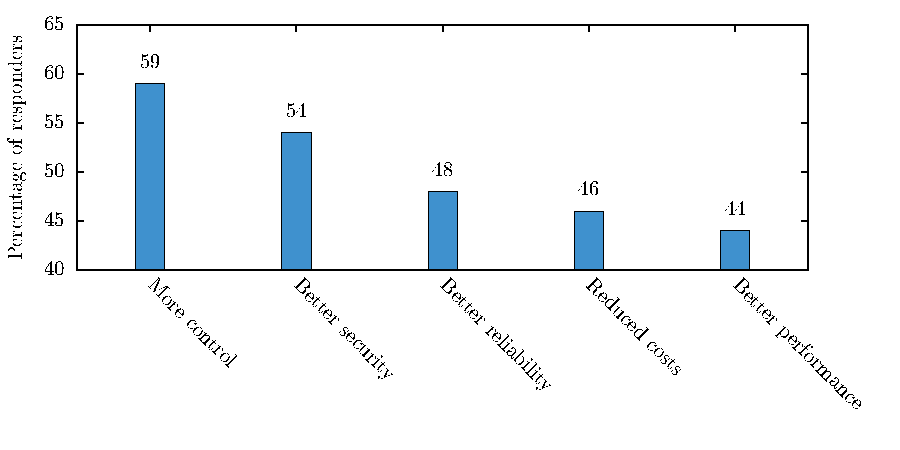
\includegraphics{chapter-interoperability/hybrid-cloud-top-benefits}
  \end{center}
  \caption{Top benefits of using the hybrid model according to \cite{RackspaceSurvey13}}
  \label{fig:hybrid-cloud-top-benefits}
\end{figure}

\section{Federation of clouds -- InterCloud}
As stated in the previous sections, one of the major obstacles that prevents consumers from adopting cloud solutions is reliability. It appears that these statements are not only imaginary worries of entrepreneurs, but real problems -- there are cases, where some providers temporarily run short of capacity (e.g. because of provisioning too many virtual machines) in the face of hight demand \cite{Lavitt09}. What is more, the more demanding clients require specific QoS to be satisfied by their providers as negotiated in Service Level Agreements.
In order to meet these challenges there is a need of a completely new approach to the problem of effective management of resources. The new solution should take into account such factors as:

\begin{itemize}
  \item users' requests priority
  \item users' QoS requirements (e.g. the deadline by which some jobs have to be executed)
  \item price that the clients pay for the usage of resources
\end{itemize}

Computer scientists in the field of cloud computing devised a model \cite{MarketOrientedCC08} in which resources are managed in a market-oriented fashion that enables dynamic regulation of the supply and demand of resources and promotes the mechanisms for their allocation that would take into account their priorities and levels of utilization.
The extension of this model is a vision of creating the federated cloud computing environment, so called \emph{InterCloud}, that ``facilitates just-in-time, opportunistic, and scalable provisioning of application services, consistently achieving QoS targets under variable workload, resource and network conditions'' \cite{InterCloud10}.
The elements of the proposed architecture are as follows:
\begin{itemize}
  \item Cloud Exchange -- acts as a market maker for bringing together both producers and consumers of services. It allows Cloud Brokers and Cloud Coordinators to match consumers with the fitting offers from providers. Such a market is a step forward towards creating a dynamic infrastructure for trading based on Service Level Agreements.
  \item Cloud Coordinator -- manages the instance of a cloud and its membership in the overall federation; provides an environment (programming, deployment) for applications
  \item Cloud Broker -- acts on behalf of the client; communicates with the Cloud Exchange to find the best cloud instances for the application
\end{itemize}

\subsection{Usage in industry}
The depicted model has not yet been adopted in the industry, yet some simulations were carried out on a \emph{CloudSim} platform and the obtained results showed that this concept has ``immense potential'' \cite{InterCloud10}.


\chapter{Related work} 

\chapterintro{This chapter presents recent achievements in a field of platform-as-a-service model by examining: Carina, OneFlow, CloudFoundry and OpenShift. Especially, it focuses on aspects of adaptivity, scalability and cloud federation awareness.}

\section{Requirements}
One can notice that elements that yields a solution to a problem stated in the first chapter, which is ensuring that users' application provide appropriate Quality-of-Service for its customers in a most-cost effective manner, were gradually introduced in previous chapter:

\begin{itemize}
	\item \emph{adaptivity} - ability to adapt (i.e. scale) appropriately to a current usage pattern
	\item \emph{scalability} - ability to improve application performance by enriching resources
	\item \emph{cloud-federation awareness} - ability to compose an application deployment using different cloud providers; cooperation with different cloud provider to supply application with extra resources while performing application scaling
\end{itemize}

In the next sections we examine latest advancements used by a platform-as-a-service providers that is: Carina, OneFlow, CloudFoundry and OpenShift. Apart from getting into detail regarding above-mentioned factors, we scrutinise whether given product satisfies following functional and non-functional requirements. 

\subsection{Functional requirements}
\begin{enumerate}
  \item The user of the platform is able to:
    \begin{enumerate}
      \item deploy a service,
      \item cancel the service,
      \item check the status of the previously ordered-to-deploy service at any time. \emph{Status} means 
        \begin{inparaenum}[a)]
        \item whether or not the deployment succeeded,
        \item current uptime of the service,
        \item current cost
        \end{inparaenum}
    \end{enumerate}
  \item One of the elements of the platform is a client application that is used by the user of the platform to communicate with it,
  \item During the deployment process, the platform takes as an input a description of the service (application) that consists of:
    \begin{itemize}
    \item service name,
    \item software stacks (e.g. \emph{java}, \emph{ruby}),
    \item scaling policies (per each stack) which define
      \begin{inparaenum}[i)]
      \item minimal and maximal number of VMs that are needed for the stack,
      \item name of the policy (algorithm) which is used for scaling,
      \item parameters of the policy
      \end{inparaenum}
    \end{itemize}
  \item Deployment of a service is done in a way which minimizes the cost from the client's perspective with ensuring Quality-of-Service requirements at the same time,
  \item The platform monitors the state of the deployed services and based on the results of this process takes appropriate steps in order to meet the auto-scaling requirements. These include
    \begin{inparaenum}[a)]
    \item altering VM's parameters and configuration,
    \item vertical scaling,
    \item horizontal scaling,
    \item scaling stacks among different cloud providers
    \end{inparaenum}
\end{enumerate}

\subsection{Non-functional}
\begin{itemize}
  \item The platform does not confine itself to one provider, but to a \emph{ecosystem of various cloud providers} that offers deployment capabilities which vary in terms of quality of service, cost, etc.
\end{itemize}
	
% radek
\section{Carina}

\subsection{Introduction}
Carina is an open source project, released under Apache License 2.0, built on top of OpenNebula, which aims to ``(\ldots) standardize the process for automating multi-VM deployments and setting auto-scaling and availability management policies in the cloud.'' \cite{CarinaBlog}. The project is used by the authors at their work at RIM in an OpenNebula-based private cloud.

\subsection{Features}
As it is stated in the requirements of the solution, \emph{Carina} should support variety of features which can be considered worth scrutinizing carefully as they are closely related to notions of adaptivity and scalability. To name the most relevant: \cite{CarinaBlog}
\begin{itemize}
  \item Collect and aggregate OS or app-specific metrics across a cluster
  \item Drive elastic scaling of clusters based on workload or events
  \item Support deployment and handling of failover of services across multiple datacenters
\end{itemize}

Before delving into more detailed description it is vital to introduce most important terms used in \emph{Carina} documentation to depict this product:
\begin{itemize}
  \item Environment -- a collection of VMs in a master-slave configuration,
  \item Service -- a consumer of cloud resources. Each service can have its own environment configurations and create environments and control them independently of other services,
  \item Pools -- various clusters or virtual data centers in OpenNebula that can be targets for creating an environment
\end{itemize}

\subsection{Key technical concepts}

\subsubsection{Adaptivity}
In \emph{Carina} there are mechanisms which can perform application scaling, both in manual and automatic fashion. It is possible for a system administrator to directly modify the existing application and its environment by changing its parameters manually. Automatic management of an environment is done by defining \emph{scaling policies} which can be in two flavours: \emph{time-based} and \emph{load-based}. Those are called by the authors \emph{elasticy policies}.

\emph{Time-based} policies defines how the system should react in the given window frame(s). In each frame we can specify the minimum number of virtual machines that comprises an environment. On the other hand, \emph{load-based} policies define the way the system reacts to \textbf{average cpu usage} by the environment. This is the simplest \emph{threshold-model} as introduced in chapter 2. The user enters predicates which are evaluated against data gathered by OpenNebula and execute scaling actions  (\emph{scaleup} and \emph{scaledown}) if they are true. What is more, the minimal and maximal number of virtual machines must be specified. At present the only parameter that is taken into account while performing actions triggered by \emph{load-based} policies is cpu usage.

To increase the application availability, \emph{Carina} introduces the notion of \emph{availability policies}. Their main function is to take a recovery action in response to a deletion or errors during deployment of a virtual machine. Recreation of a virtual machine is the most fundamental and atomic operation under this model.

\subsubsection{Scaling}
Chapter 3 introduced and discussed various types of application scaling. \emph{Carina} offers only one type of scaling and this is \emph{horizontal} scaling -- user's capabilities are limited only to add/remove a virtual machine to/from a given environment. Unfortunately there are no means to modify the parameters of a given or a set of virtual machines.

\subsubsection{Cloud federation awareness}
In this paper we strongly advocate spanning cloud resources across multiple vendors/providers. Despite having in its requirements such a position, \emph{Carina} \textbf{does not} support deployment or scaling of services across different providers. In the environment configuration we define only \textbf{one} endpoint -- this is can be thought of a reference to a cloud provider. As it can be only one per environment, it is not possible to deploy or scale some artifacts across many providers.

\subsection{Design}
To complete the discussion about \emph{Carina} it is essential to include its architecture overview. This is shown in figure \ref{sota:carina-design}.

\begin{figure}[!ht]
  \begin{center}
    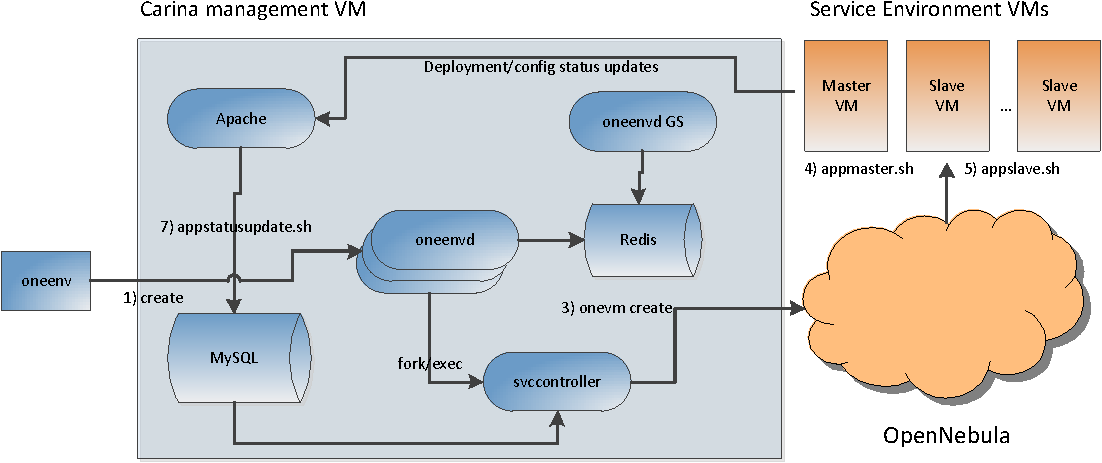
\includegraphics[width=\textwidth]{chapter-state-of-the-art/carina-design}
  \end{center}
  \caption{Carina -- components interaction}
  \label{sota:carina-design}
\end{figure}

There are number of things that cause concern:
\begin{asparaenum}
\item[\textbf{Persistency}] No one knows for what reason, but \emph{Carina} uses two databases. What makes things even worse, they completely differ in types, as \emph{MySQL} is a relational and \emph{redis} is a nosql database. This places additional burden on technical requirements of the platform.
\item[\textbf{Usage of Apache}] To work properly, \emph{Carina} needs Apache http server. In the server cgi-bin directory there are placed bash scripts which are invoked by contextualization scripts executed in different stages of virtual machines life cycle. Instead, we recommend setting proper web services, environment-agnostic, in a central node which can be run next to global scheduler.
\item[\textbf{User accounts}] \emph{Carina} forces the creation of a system-wide user for each service. These concepts should be totally independent.
\item[\textbf{Provisioning}] User has to use in the environment specification previously defined OpenNebula images. Their further adjusting happens in the contextualization phase. This forces the user to modify the state of a virtual machine when there is a need to perform any changes, for example in the software stack. Instead we suggest using some provisioning software such as puppet or chef -- this would enable users to change software stack only in configuration files (recipes) not by altering the virtual machine state.
\end{asparaenum}

\subsection{Summary}
\emph{Carina} emerged as a promising platform built on top of OpenNebula, which lacked most of its functionalities at that time. The good point is the fact that this product is used in a business context and judging by the authors' description it actually works. However, due to deficiencies mentioned in the previous sections, \emph{Carina} cannot be considered a mature and generic solution for more demanding cloud providers.



\section{OneFlow}

\subsection{Introduction}
\emph{OneFlow} \cite{OneFlow} is a management system integrated into \emph{OpenNebula} that aspires to enhance it with multi-tiered applications (service) deployment and auto-scaling capabilities. It is available as a core part of \emph{OpenNebula} since 4.2 version and released under \emph{Apache License, Version 2.0}. 

\subsection{Features}
In a context of this thesis, \emph{OneFlow} enriches \emph{OpenNebula} with only one, yet powerful feature: application scaling based on policies. Besides this, benefits of using \emph{OneFlow} are as follows:
\begin{itemize}
\item defining multi-tiered applications (services) as a collection of applications
\item providing configurable services from a catalogue and self-service portal
\item enabling tight, efficient administrative control
\item fine-grained access control for the secure sharing of services with other users
\end{itemize}

\subsection{Key technical concepts}
\subsubsection{Adaptivity}
Adaptivity is achieved by specifying policies, that violated, trigger events impacting service environment. There are two types of policies available:
\begin{itemize}
 \item \emph{Auto-scaling based on metrics} - policy defines an expression that triggers scaling adjustments. Expressions can use performance data sent from virtual machine using \emph{OneGate} as well as virtual machine data such as CPU, memory, network bandwidth
 \item \emph{Auto-scaling based on schedule} - policy specifies a time or a time recurrence and correlates that information to appropriate service adjustments
\end{itemize}

Apart from scaling policies, scaling is controlled by a minimal and maximal number of virtual machines that can compose a service.

\subsubsection{Scaling}
\emph{OneFlow} is capable of \textbf{only} horizontal scaling: it adds or removes virtual machine using \emph{OpenNebula API}, when appropriate event is triggered. Violating given policy results in virtual machine's state transition into \texttt{SCALING}. After proper action is finished, virtual machines converges to a \texttt{COOLDOWN} state. What this simple state transition does is allows an environment to accommodate changes and adjust to a recent changes, disabling scaling for a given period of time.


\subsubsection{Cloud federation awareness}
\emph{OneFlow} itself \textbf{does not} cooperate with different cloud instance. Hence, one is limited to \emph{OpenNebula} hybrid or public cloud capabilities that employs oZones and \emph{AWS}, respectively. Although, they expand single \emph{OpenNebula} instance capacity it is limited in a way that discriminates it as possible solution. Firstly, the problem with oZones is that they require centralised management, while cloud federation is by definition distributed and independent. Secondly, cloud bursting into \emph{AWS} limits instance monitoring capabilities. Consequently, it is not possible to supervise provisioned instances.

\subsection{Summary}
Taking everything into consideration, OneFlow is a valuable addition to OpenNebula ecosystem. Undoubtedly, its auto-scaling feature with elastic policy mechanism cannot be underestimated. However, actions taken by scaling mechanism are coarse-grained by being limited to a horizontal scaling. What makes things worse, OneFlow can not leverage resources of multiple providers associated within a cloud federation.

\section{OpenShift}

\subsection{Introduction}
\emph{OpenShift} is developed by \emph{RedHat} Platform-as-a-Service solution. It is available in two different flavours:
\begin{itemize}
 \item \emph{OpenShift Enterprise} (private cloud)
 \item \emph{OpenShift Online / FreeShift} hosted by RedHat (public cloud)
\end{itemize}

The latter is freely distributed, but it is limited to only 3 gears (a 'gear' is a resource maintained by \emph{OpenShift}, such as application server or database). Beside this, source code is hosted on github and licensed under \emph{Apache License 2.0}.

\subsection{Features}
High level features that distinguishes \emph{OpenShift} are as follows:
\begin{itemize}
  \item accelerated application service delivery by on-demand and self-provision application stack access
  \item minimised vendor lock-in by portability (there are no proprietary APIs, technologies)
  \item automatic application scaling
\end{itemize}

Beside this, key qualities include:
\begin{itemize}
  \item polyglot stacks: there is a number of built in application stacks (Java, Ruby, Python, databases); user is allowed to defined one himself through a concept of 'cartridge'
  \item one click deployment: application are managed by \emph{OpenShift} through git repository. Deploying new version of application comes down to pushing new version application's source code.
  \item SELinux-based secure containers for multi-tenancy
  \item automatic application stack provisioning, it is only necessary to specify required cartridge (application stack) and all the dependencies are provided by platform
\end{itemize}

\subsection{Key technical concepts}

\subsubsection{Adaptivity}
\emph{OpenShift}'s adaptivity capabilities are constrained to a simple case: while creating a new application, it is possible to specify whether application should scale. As a consequence, additional gear is allocated to serve \emph{HAProxy} \cite{HAProxy}. There is only \textbf{one built-in} scaling policy that is based on a relatively straightforward algorithm \cite{OpenShiftScaling}:
\emph{\begin{quote}
The algorithm for scaling up and scaling down is based on the number of concurrent requests to your application. OpenShift allocates 10 connections per gear - if HAProxy sees that you're sustaining 90\% of your peak capacity, it adds another gear. If your demand falls to 50\% of your peak capacity for several minutes, HAProxy removes that gear.
\end{quote}}

\subsubsection{Scalability}
As previous point implies, OpenShift \textbf{solely} uses horizontal scaling: it adds additional gears if number of requests increases beyond certain level.

\subsubsection{Cloud federation awareness}
OpenShift does not use any notion of a cloud provider or datacenter. However, since cartridges are in fact Linux processes running on OpenShift Nodes, it is possible to deploy  OpenShift Enterprise on any infrastructure running RHEL. It can consist of physical nodes as well as virtual machines, managed, for example, by OpenStack. With all that said, is still requires a centralised, OpenShift controlled environment. Hence, OpenShift \textbf{is not} capable to work in a cloud federation.

\subsubsection{Multi-tenancy}
In OpenShift, each application is represented as a set of gears. For example, gear is a database or application server. Gears are hosted on OpenShift Nodes. There is a many-to-one relationship between gear and OpenShift Nodes. What is leveraged to achieve this multi-tenancy is:
\begin{itemize}
 \item SELinux, isolation between applications running at the same node
 \item control groups (cgroups), fine-grained control over the memory / CPU / IO utilisation / networking on per process basis
 \item kernel namespaces, groups of processes are separated, so that they cannot see resources in other groups
\end{itemize}

\subsection{Summary}
Summing up, key advantage of the OpenShift seems to be it simplicity: creating and deploying applications using OpenShift is as simple as it gets. Beside this, built in support for most popular technologies and simple API makes OpenShift attractive platform. Having that said, oversimplified auto-scaling and being constrained to a single cloud provider may be not sufficient in complicated scenarios.

% radek
\section{CloudFoundry}
\subsection{Overview}
\emph{Cloud Foundry} is a platform-as-a-service solution which can be installed on local or off-premises infrastructure, such as Amazon Web Services, OpenStack or vSphere. It is available in two versions as
\begin{itemize}
  \item an open-source project
  \item a commercial solution, \emph{Pivotal CF}
\end{itemize}
In this section we want to elaborate only on an open-source project.

\subsection{History}
The project was initially developed by VMWare and its first release was in 2011, It was then that VMware decided to make it available to the general public and released it under Apache License 2.0. For the next consecutive two years, there were maintained two versions of \emph{Cloud Foundry} -- as a hosted solution owned by VMWare and an open-source project. However, in December 2012 VMware and EMC shared information on the \emph{Pivotal Initiative} \cite{PivotalInitiative} -- a virtual organization of people from both companies with background in \emph{big data} and \emph{cloud application platforms}. With the advent of the this new entity, \emph{Pivotal} \cite{GoPivotal}, it was announced the launch of the new product -- Pivotal One, which is powered by \emph{Pivotal CF}, the enterprise version of \emph{Cloud Foundry}. Now users can choose between the open-source and commercial solutions.

\subsection{Features}
Below there are listed some of the main functionalities offered by \emph{Cloud Foundry}:
\begin{itemize}
  \item Support for multi-provider ecosystem (\emph{Multi-Cloud})
  \item Reduced the management burden of the life-cycle of an application by a simplified CLI that enables, e.g. faster and instant deployment,
  \item Dynamic routing which enables and enhances horizontal scaling and updating applications,
  \item Usage of own-developed lightweight containers (\emph{Warden}), which ensures the proper isolation level and improves the speed of movement of application instances between virtual machines (utilizing \emph{aufs} -- advanced multi layered unification filesystem)
  \item Health management -- continually monitoring application instances and taking according recovery actions if needed
  \item Standards-based authorization and authentication system which supports various standards such as LDAP, SAML or OAuth 2.0
\end{itemize}

\subsection{Key technical concepts}

\subsubsection{Cloud Foundry-specific}
\begin{asparaenum}
\item[\textbf{Warden}] The main goal of \emph{Warden} is to manage isolated and resource-controller environments called containers. It is responsible for management of the whole lifecycle of an environment and provides API for actually performing any operation on a container. At first, \emph{Warden} used LXC technology under the hood, but now containers are an own product of \emph{Cloud Foundry} community.
\item[\textbf{Droplet Execution Agent}] \emph{DEA} manages \emph{Warden} containers, stages user's application and runs droplets -- wrappers around already deployed applications.
\item[\textbf{BOSH}] \emph{BOSH} is a tool chain for release, deployment and lifecycle management of distributed services. Its functionalities can be compared to those offered by \emph{Chef}.
\end{asparaenum}

\subsubsection{Adaptivity}
\emph{Cloud foundry} does not support auto-scaling -- it is only possible for the cloud consumer to scale the application manually. However, there can be additional tools which can add this functionality, such as \emph{RightScale}.

In terms of monitoring the state of applications, the platform uses \emph{Health Manager} to collect relevant data and then it notifies \emph{Cloud Controller}, which in turn takes appropriate actions. This enables, for example, to spawn a new node if an existing one needs a replacement.

\subsubsection{Scalability}
\emph{Cloud foundry} supports only horizontal scaling not only within one provider, but also across many. This feature is called \emph{Multi-Cloud} in Cloud Foundry nomenclature.

\subsubsection{Cloud-federation awareness}
As it was stated in previous sections, Cloud Foundry is \emph{cloud-federation aware}, i.e. it allows users to span their applications across many providers, which results in a hybrid solution that comes in many flavours: \emph{public-public}, \emph{public-private} or \emph{private-private}.


\subsection{Summary}
Owing to the variety of useful features, great support from community and significant IT enterprises such as IBM, VMware to name a few, \emph{Cloud Foundry} can be considered a mature product which can compete with current leaders in the fields, such as Amazon AWS.
Additionally, it is highly probable that acquiring the hosted solution by \emph{Pivotal} may be of a great benefit to the whole cloud community as the market will be more competitive.

% radek
\section{Providers comparison}
In this section we would like to compare all depicted providers as well as other solution in terms of \emph{adaptivity} and \emph{scalability} as none of the examined providers support \emph{cloud federated} deployments. Table \ref{tab:cloud-providers-scaling} presents a summary of cloud providers auto-scaling capabilities. Interestingly, all of them are focused solely on horizontal scaling, ignoring advantages offered by a fine-grained approach to scaling that leverage scaling up and application tuning. Table \ref{tab:cloud-providers-adaptivity} summarises platforms approach to adaptivity: their data analysis mechanisms and policies support.

\begin{table}[!htbp]
\begin{tabularx}{\textwidth}[]{ X  X  X  X}
\specialrule{.1em}{.05em}{.05em} 

  & \textbf{Horizontal scaling} & \textbf{Vertical scaling} & \textbf{Application tuning} \\
\specialrule{.1em}{.05em}{.05em} 

\multicolumn{4}{ l }{\textbf{Infrastructure provider}} \\
\specialrule{.1em}{.05em}{.05em} 

Carina & \checkmark & $\times$ & $\times$ \\ \hline

OneFlow & \checkmark & $\times$ & $\times$ \\ \hline

AWS EC2 & \checkmark & $\times$ & $\times$ \\ \hline

\multicolumn{4}{ l }{\textbf{Platform provider}} \\
\specialrule{.1em}{.05em}{.05em} 

CloudFoundry & $\times$ & $\times$ & $\times$ \\ \hline

OpenShift & \checkmark & $\times$ & $\times$ \\ \hline

AppEngine & \checkmark & $\times$ & $\times$ \\ \hline

Azure & \checkmark & $\times$ & $\times$ \\ \hline

Heroku & $\times$ & $\times$ & $\times$ \\ \hline
\end{tabularx}

\caption{Comparison of cloud providers scaling capabilities}
\label{tab:cloud-providers-scaling}

\end{table}


\begin{table}[!htbp]
\begin{tabularx}{\textwidth}[]{ X  X X }
\specialrule{.1em}{.05em}{.05em} 

  & \textbf{Policies} & \textbf{Data analysis} \\
\specialrule{.1em}{.05em}{.05em} 

\multicolumn{3}{ l }{\textbf{Infrastructure provider}} \\
\specialrule{.1em}{.05em}{.05em} 

Carina & 
-- time frame based

-- expression based (only for CPU)
&
-- threshold model that takes into account minimal and maximal permitted instances of an application as well as application priority

\\ \hline

OneFlow 4.2 & 
-- time frame based with customizable padding 

-- expression based build on custom language, where all vm's metrics are supported

-- customizable adjustment padding, cooldown time
&
-- threshold model

\\ \hline

AWS EC2 & 
-- time frame based

-- expression based, where expressions corresponds to a AutoScalingGroup

-- actions are triggered by a CloudWatch alarms

-- customizable adjustments paddings, types, cooldown time
&
-- threshold model, takes into account minimal and maximal permitted instances of an application as well as application priority
\\ \hline

\multicolumn{3}{ l }{\textbf{Platform provider}} \\
\specialrule{.1em}{.05em}{.05em} 

CloudFoundry & $\times$ & $\times$ \\ \hline

OpenShift & 
-- single built-in policy

 &
-- single built-in threshold model that scales an application when CPU load is greater than 50\% for a given period
\\ \hline

AppEngine & 

-- built-in policy based on request queue length

-- adjustable minimal, maximal number of application instances, pending latency

 &
-- queue-based, new instance is provisioned if queue length got too long 
  \\ \hline

Azure & 
-- time frame based

-- expression based, where expression can involve either CPU usage or Queue length

-- customizable adjustments paddings, types, cooldown time
&
-- threshold model, that takes into account minimal and maximal allowed instances
 \\ \hline

Heroku & $\times$ & $\times$ \\ \hline
\end{tabularx}

\caption{Comparison of cloud providers approach to adaptivity}
\label{tab:cloud-providers-adaptivity}

\end{table}





\chapter{Cloud-SAP}

\chapterintro{ This chapter introduces the reference architecture known as Cloud-SAP, highlights its core concepts and indicates possible implementation ideas.
}

\section{Motivation}
As one can see, latest advances in providing platform-as-a-service still do not yield a comprehensive solution that embraces a range of fine-grained actions relevant to a given situation in an environment, as it was summarised in previous chapter. All of the presented solutions solely engage horizontal scaling, while other IT processes and corresponding actions such as vertical scaling, cloud bursting or application platform restart remains neglected. What is more, none of the investigated systems take proactive approach in enforcing given QoS.

What has all of the above-mentioned features is a self-adaptive system that has a holistic approach to an application scaling. As \cite{brun2009engineering} advocates, one of the first architectures of a self-adaptive system was presented in IBM's blueprint for autonomic computing \cite{IBM06}. IBM's autonomic system is widely recognised and respected and hence we decided to leverage it as a foundation of our work. A concept of autonomic system is alluring due to its four crucial attributes:
\begin{itemize}
 \item \emph{self-configuration} - dynamic adaptation to changing environment such as provisioning new application instances, application tuning, traffic delegation to an external provider
  \item \emph{self-healing} - discovering, diagnosing and reacting to environment disruption such as container outage
  \item \emph{self-optimising} - monitoring and tuning resources: migrating containers, offloading traffic, for example
  \item \emph{self-protecting} - detecting and protecting against threats such as Deny-of-Service by provisioning extra resources
\end{itemize}

These four system capabilities combined together yield a promising architecture from QoS ensuring perspective. Beside this, key customer values such as IT process execution cost or time needed to complete it are enhanced through rapid process initiation and reduced time and skill requirements \cite{IBM06}. As specified in blueprint, applying autonomic system to manage application environment is possible because following conditions are met:
\begin{itemize}
  \item tasks involved in associated IT process needs to be automated
  \item it is possible to initiate processes based on observable and detectable situations
  \item autonomic manager posses sufficient knowledge
\end{itemize}

Cloud Self Adaptive Platform (Cloud-SAP) is a reference architecture aspiring to supply application providers with a self-adaptive computing environment. Figure \ref{img:csap-usage-context} shows Cloud-SAP place in an exemplary application provisioning request. 
\begin{figure}[!ht]
  \begin{center}
    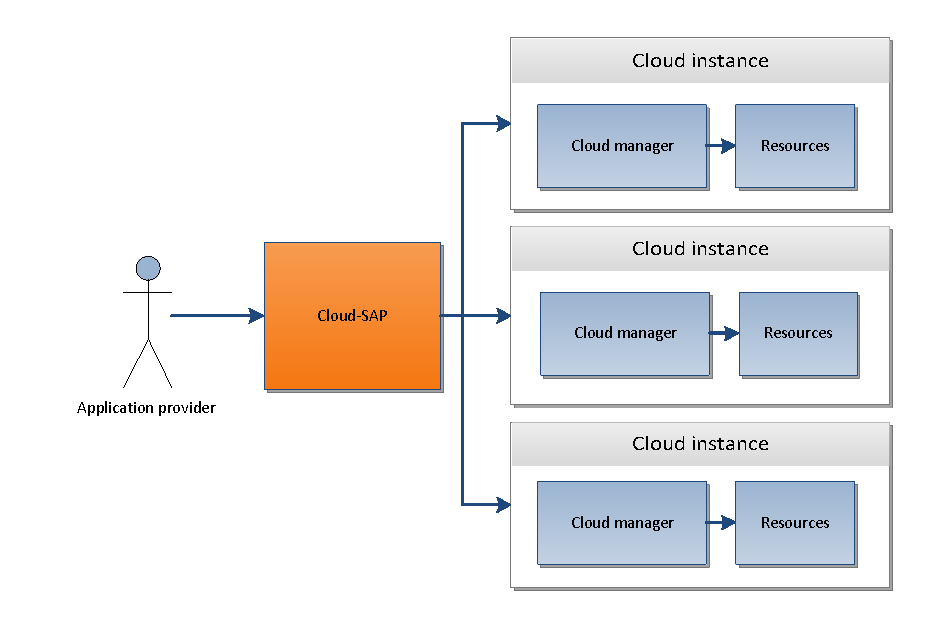
\includegraphics[width=0.9\textwidth]{chapter-design/csap-usage-context}
  \end{center}
  \caption{Cloud-SAP place in an exemplary application provisioning request}
  \label{img:csap-usage-context}
\end{figure}

Application providers can be both end-users or other system interfaces, Cloud-SAP is suitable for both cases. Cloud-SAP is entirely cloud provider and resource agnostic as long as they externalise management interfaces.

Successive sections define core layers of a Cloud-SAP and give insight into possible implementation decisions, while the next chapter presents a proof-of-concept implementation. While proposed architecture yields a self-adaptive system not an autonomic one, it is based on such model and hence we use terms characteristic to that kind of system as presented in IBM's paper \cite{IBM06}.

\section{Overview}
The previous section dealt with all premises that led to a conclusion that the proposed architecture can rely heavily on the concept of an autonomic system. In this section the further elaboration on the solution is presented.
Figure \ref{img:csap-usage-context} showed the context which the architecture applies to. As one can see, Cloud-SAP can be seen as a proxy between the user and cloud instances and as a coordinator of the latter. Although the cloud instance itself consists of a cloud manager and additional resources, in general, it is perfectly legitimate to consider it a resource as well. 

Before the more detailed diagram of the solution is presented, it is essential to introduce another indispensable function that lies in the heart of any autonomic entity -- its ability to detect an undesirable state and take appropriate actions. This is achieved by the presence of a \emph{control loop} which collects data about the environment, analyzes it and takes all needed steps to recover the system. Not only can the attributes introduced in the previous section be bound to an autonomic system, but they can also be thought of main and broad categories of a control loop \cite{IBM06}.

Having said so, we are ready to give a layered overview of a proposed solution, which is shown in figure \ref{img:csap-layered-structure}.
\begin{figure}[!ht]
  \begin{center}
    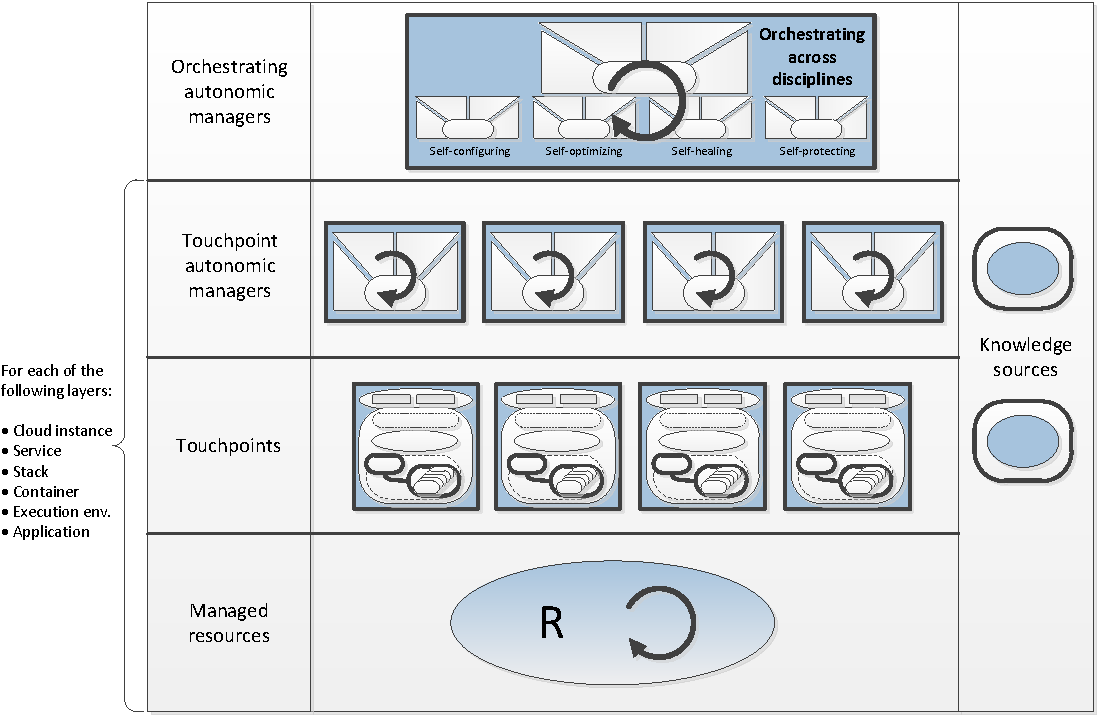
\includegraphics[width=\textwidth]{chapter-design/csap-layers}
  \end{center}
  \caption{Cloud-SAP components seen as IBM autonomic system \cite{IBM06}}
  \label{img:csap-layered-structure}
\end{figure}

The building blocks of the architecture are:
\begin{itemize}
  \item Managed resources
  \item Touchpoints
  \item Touchpoint autonomic managers
  \item Orchestrating autonomic managers
  \item Knowledge source
\end{itemize}
As resources were identified on various levels of abstraction, starting from the application that is to be deployed and ending on a cloud instance that aggregates different applications and services, we can think of the last three layers (managed resources, touchpoints and touchpoint autonomic managers) as a one logical component which can aggregate and manage other components. This recursive definition applies to identified managed resources described in the next section, apart from application as we consider it the most fundamental and indivisible resource.

\subsection{Managed resources}
\emph{Managed resources} form the lowest layer of a stack. When it comes to application provisioning in a cloud environment we can think of the following resources:
\begin{itemize}
  \item \emph{Application} - application itself can be considered resources which can be managed by an external entity, e.g. by restarting/killing it. Interestingly, an application itself can be an autonomic component with an embedded control loop. However, such setting is completely transparent to Cloud-SAP and therefore cannot be managed by it.
  \item \emph{Execution environment of an application} forms an inherent part of an application lifecycle and its proper tuning can greatly influence its performance,
  \item \emph{Container} -- an isolated and controlled environment in which applications are deployed,
  \item \emph{Stack} -- every application has a technology stack associated with it; what is more, if we confine ourselves to map one instance of a container with only one application, we can think of stack as a composition of application (and its execution environment) and a container,
  \item \emph{Service} -- more complex solutions/applications require interactions with various components that are not necessarily implemented using the same technology stack; service denotes a logical entity that consists of a list of stacks that should form one, indivisible component,
  \item \emph{Cloud instance} -- an entity able to deploy \emph{services}
\end{itemize}
What is more, the listed resources are nested within one another and one's ability to work/run smoothly highly depends on the condition and state of the resource it forms part of. This is shown in figure \ref{img:managed-resources-aggregation}.
\begin{figure}[!ht]
  \begin{center}
    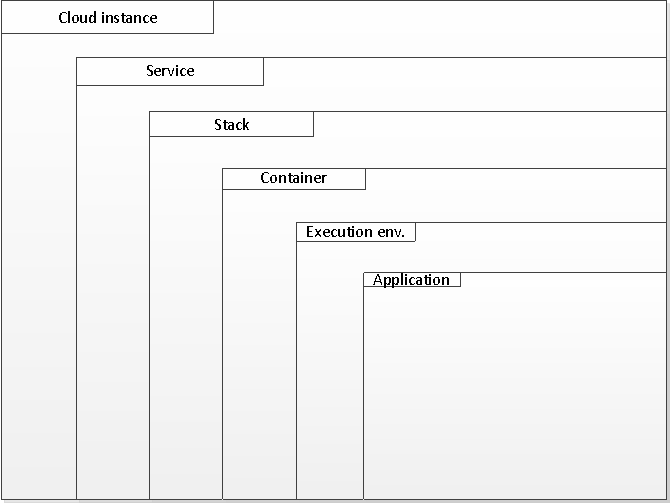
\includegraphics[width=\textwidth]{chapter-design/csap-resources-aggregation}
  \end{center}
  \caption{\emph{Managed resources} identified by Cloud-SAP and their aggregation}
  \label{img:managed-resources-aggregation}
\end{figure}

As it is shown in figure \ref{img:csap-layered-structure}, each \emph{managed resource} can have embedded self-management control loop. The control loop may or may not be externally visible by the manageability interface. For example, an application can have \emph{self-configuring} control loop which performs appropriate runtime tuning of its configuration files, while not being visible (by not providing any API) and manageable by any entity.

\subsection{Touchpoints}
\emph{Touchpoint} forms the layer above managed resources. It has two main functions \cite{IBM06}:
\begin{inparaenum}[1)]
\item provide manageability interface and
\item implement \emph{sensor} and \emph{effector} behaviour.
\end{inparaenum}

By means of manageability interface, external entities can control managed resources. It can be done by, e.g. leveraging API, configuration files or logs. Additionally, it is possible to obtain information via touchpoint about the state of the resource. \emph{Sensor} and \emph{effector} behaviours refers to mechanisms that allows collecting data and change the behaviour of the resource, respectively. Structure of touchpoint is shown in figure \ref{img:csap-touchpoint}.

\begin{figure}[!ht]
  \begin{center}
    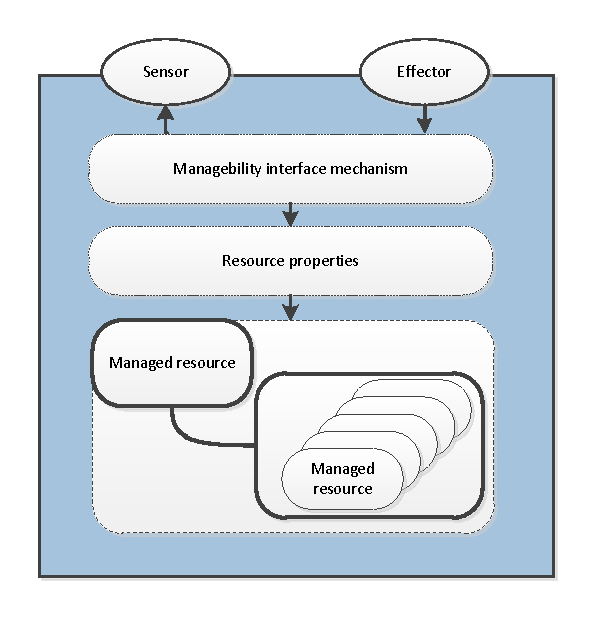
\includegraphics[width=0.7\textwidth]{chapter-design/csap-touchpoint}
  \end{center}
  \caption{Touch point component}
  \label{img:csap-touchpoint}
\end{figure}

\subsection{Touchpoint Autonomic Manager}
\emph{Touchpoint Autonomic Manager} is a component that implements the control loop behaviour and, in effect, manages the managed resources through exposed touchpoints. As it was stated in the previous sections, only four types of control loops are of an interest in the proposed architecture, i.e. \emph{self-configuring}, \emph{self-healing}, \emph{self-optimising} and \emph{self-protecting}.

The actions executed by each control loop on the assigned managed resource are defined in a \emph{policy} that is associated with the given autonomic manager. Thus, there is a one-to-one mapping between managed resource and touchpoint, and touchpoint and autonomic manager.

Each autonomic manager implements the control loop which can be split into four consecutive blocks, which share knowledge among one another. The output from one block forms an input to another. However, it is perfectly possible for a block to perform an action for obtaining side effects, e.g. an action can result in producing relevant information contained in log files, which, in turn, comprises a piece of shared knowledge. Each block implements different behaviour based on the abstraction level and resource they operate on (see figure \ref{img:csap-layered-structure}). Nevertheless it is possible to define their generic behaviour, which embraces the four phases: monitoring, analysis, planning and execution.

\subsubsection{Monitoring}
This function of autonomic manager is responsible for collecting and aggregating data about the resource it manages.  While Cloud-SAP does not have any specific requirements regarding underlying monitoring mechanism, there are a few aspects that should be taken into consideration:
\begin{asparaenum}
  \item[\textbf{Metrics}] Whilst there is a variety of metrics describing resource state, there is no point in monitoring data that client is not interested in. For example, in case when client-defined policies rely entirely on CPU measurements, memory or bandwidth is irrelevant.

  \item[\textbf{Data filters}] Provided that data is gathered from a resource, not all of it should be analysed as some portion of it may be distorted. More specifically, there may be some random spikes in measurements, caused by a temporary process such as garbage collecting. Therefore, Cloud-SAP recommends to transform data using aggregation functions like average, median or filter by apply low or high-pass filters.

  \item[\textbf{Persistence}] Should collected data be used as a reference point during future control loop iterations, it is persisted along with measures applied by an executor. As a consequence, successive assessments can be more effective by taking into account past symptoms and configuration adjustments. Decision whether to store data in databases, files, external location is entirely left to an implementation.

  \item[\textbf{Standard compatibility}] Whilst there is no single, industry accepted standard of monitoring above-mentioned resources that range from a single application to whole cloud instance, there were initiatives such as OCCI \cite{OCCI} that aims to close that gap and provide unified view of common appliances. Having scaling across multiple cloud instances in mind, it is vital to provide compatibility at a monitoring level. However, in some cases, standard-defined API may no be sufficient for a specific needs. 
\end{asparaenum}

\subsubsection{Analysis}
This part takes the data from \emph{monitor} phase and performs in-depth analysis of it, which can result in, e.g. prediction plans. It is possible to incorporate more complex mechanisms (e.g. machine-learning) to better use the available information. For example one or more of the following models can be leveraged \cite{LiWoZh05}:
\begin{asparaenum}
 \item[\textbf{Queue-based performance models}] This models aims to predict QoS measures using resource state and environmental disturbances such as number of service requests. Then a configuration satisfying given QoS is found by a search technique using queues and layered queues. 
 \item[\textbf{Dynamic models}] Aims to represent QoS as a cost function of the difference between the measured value from sensors and value set by effectors. Model aspires to minimize that function. Linearized dynamic control is an example of a dynamic model. 
 \item[\textbf{Monotonic static models}] Sought resource state is calculated by discretising a performance model or performing heuristic principles in performance engineering. 
 \item[\textbf{Error correction}] Analysis precision can be improved by applying paddings based on historical data:
    \begin{itemize}
      \item \textit{Burst based padding} - employs a signal processing technique based on fast Fourier transform, burst pattern is extracted and used to calculate a padding value. Coefficients that represents the amplitude of each frequency component are used to calculate burst density. Depending of that value (i.e. is higher than 50\%) appropriate percentile of the burst values are used \cite{ShSuGuWi11}  
      \item \textit{Remedial padding} - padding errors are being recorded and used in successive padding evaluations. In other words, let $e_1, e_2, ... e_k$ denote the recent prediction errors, next the weighted moving average is calculated. Actual applied padding is either padding itself or weighted average, depending which one is greater \cite{ShSuGuWi11}    
    \end{itemize}
 \item[\textbf{Policy based models}] Policy is expressed as a set of constraints that characterise needed resource state. Policies can be categories into two types:
    \begin{itemize}
     \item \emph{Threshold control} - it was already discussed and illustrated in figure \ref{fig:threshold-model}. For example, CPU load can be monitored and when it exceeds a given value, CPU share is increased.
     \item \emph{Policy function control} - a mutli-dimensional extension of a threshold model. It uses multiple variables and control levels \cite{abdeen2002seeking}. It can be further optimised by using Markovian model for a system behaviour \cite{ye2000markov}.     
    \end{itemize}
\end{asparaenum}
Self-learning manager should also use a predictive approach \cite{JiPeLiCh11} and track changes made in a container \cite{ZhYaWo05}. Cloud-SAP requires at least threshold-model \cite{tong1978threshold} to be supported to enable simple auto-scaling scenario.

\subsubsection{Planning}
During planning phase, procedure to enact desired state of a resource is created. Depending on problem, it may involve only one step such as adjusting one parameter or a more complex like migrating a resource. Before implementing planning module, following issues should be taken into consideration:
\begin{asparaenum}
 \item[\textbf{Priorities}] Multi-tenancy is indispensably correlated with cloud services. As a consequence, resource contends again each other to access lower-level resources. This can be mitigated by one of the following: \begin{inparaenum}[1)]
    \item avoiding over-provisioning, each tenant has guaranteed resource pool
    \item prioritise tenants, each tenant has assigned priority that indicates its business value; that priority is used to favour one tenant at the expense of the others.
 \end{inparaenum}
 
 \item[\textbf{Reservations}] As previous point indicates, different resources may have different priorities. Therefore, it is suggested to guarantee that most valuable ones have their QoS requirements satisfied by resource reservation. Inspired by a computer networks, there are at least to ways to retain a certain resource level: 
\begin{inparaenum}[1)]
    \item use parameters such as priority to favour given resource when it is not possible to content every single tenant \cite{nichols1998definition}
    \item secure in advance to retain resource throughout container lifecycle, possibly by using common history patterns \cite{braden1997resource}
 \end{inparaenum}
\end{asparaenum}

\subsubsection{Execution}
The goal of this function of autonomic manager is to execute the planned action

  
What is more, an autonomic manager exposes \emph{sensor} and \emph{effector} manageability interfaces which enables other entities (including other autonomic managers) to manage it in a similar manner as the component itself manages a resource. The image of an autonomic manager with its control loop and provided interface is shown in figure \ref{img:csap-manager}.

\begin{figure}[!ht]
  \begin{center}
    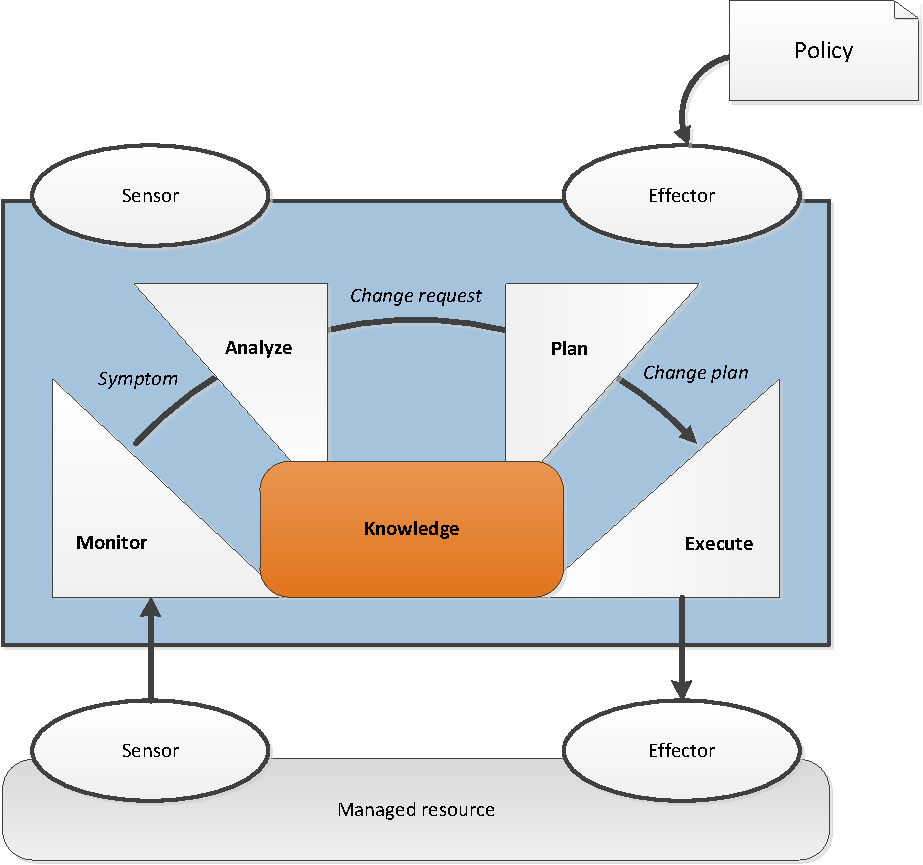
\includegraphics[width=0.7\textwidth]{chapter-design/csap-manager}
  \end{center}
  \caption{Autonomic manager}
  \label{img:csap-manager}
\end{figure}

\subsection{Orchestrating autonomic manager}
While an autonomic manager which manages a single resource may be satisfactory enough in many business cases, there are situations when additional coordination among managers is essential to attain the certain goal. This can result in incorporating autonomic behaviour within an entity in a system-wide scope.

Such a coordination can be achieved by introducing another autonomic manager whose sole purpose is to harmonize the work of dependent ones by extensive use of their \emph{sensor} and \emph{effector} interfaces. These managers are called \emph{orchestrating managers}.

When it comes to the complex task of ensuring the Quality of Service requirements for a client of a cloud computing environment, it is vital to ensure proper mechanisms that would allow seamless cooperation among different cloud providers. Such cooperation could result in a migration of an application between different clouds, market-driven choice of the cloud providers and so on.

As the exemplary actions can be regarded complex ones, they cannot be associated with actions taken by autonomic managers of only one type. Thus, an orchestrating autonomic manager should coordinate other managers of any type -- an arbitrary mixture of self-healing, self-configuring, self-optimizing and self-protecting managers. Employment of these concepts in Cloud-SAP will be discussed later in detail.

\subsection{Knowledge source}
\emph{Knowledge source} provides access to knowledge stored, for example, in a registry, dictionary or database. It is recommended that knowledge source share knowledge among multiple managers, consequently extending their capabilities by performing additional tasks: recognising particular symptoms or applying specified policies, for instance.


Whilst knowledge can be expressed as symptoms, policies, change requests or history logs, Cloud-SAP differentiates its two main types:
\begin{itemize}
 \item \emph{policy} - set of constraints that, when evaluated, influence system behaviour and possibly trigger further actions. Cloud-SAP does not specify policy format, however, it is vital to employ only one format in whole system so it can be freely exchanged
 \item \emph{problem determination knowledge} - correlation of data, symptoms and decision trees determining actions that can be taken to eliminate symptoms
\end{itemize}

An autonomic manager can obtain knowledge in one of three ways:
\begin{itemize}
 \item \emph{receive it dynamically} - a common way for passing a policy to a manager. 
 \item \emph{retrieve it from external knowledge source} - an approach for obtaining symptom definitions or historical knowledge. For example, detailed history of a resource, its problems and actions taken can be retrieved from a log file.
 \item \emph{create it dynamically} - monitoring and execution phase are strictly correlated and consequently data received from sensors, actions taken by effectors and their result can be stored as a knowledge and provide valuable information during future problem investigations
\end{itemize}


\section{Autonomic execution environment manager}
Autonomic execution environment manager supervises lifecycle of a deployed application's environment by tuning it appropriately to a given usage. More specifically it :
\begin{inparaenum}[1)]
 \item monitors application execution environment i.e. application server
 \item optimises resources used by an application such as thread pool, cache size, databases connections number
 \item restarts application when necessary
\end{inparaenum}

\subsection{Managed resource}
Application execution environment is a set of tools, APIs and frameworks that provides a generalized approach to create and run an application. It is strictly application specific. In case of java, for example, it can be represented by an application server such as Oracle Weblogic or IBM WebSphere. 

\subsubsection{Touchpoint}
Due to the fact that execution environment is so closely related to a given application type, it is not possible to enlist properties that may be exposed by a touchpoint becouse they vary from application to application. In case of Java EE application touchpoint would externalise management of thread pools, cache and JVM settings such as heap size.

\subsection{Autonomic controller}
Although autonomic controller manages a single resource - an execution environment - it in fact conducts a variety of homogeneous resources - each application type has different properties and consequently vary in actions that can be taken to optimise them. Nevertheless, following subsections presents some common issues and concerns.

\subsubsection{Monitoring}
During monitoring phase, controller collects data from execution environment's touchpoint. Depending on application type, it can involve different protocols and APIs. Should one monitor application execution environment, issues and concerns specified in overview are taken into consideration.

\subsubsection{Analysis}
Applying mathematical models to optimise application environment is an exceptionally difficult challenge due to non-linearity of a function denoting dependencies between various parameters. To make matter worse, space of possible solution is unknown and optimal solution heavily depends on a workflow that is tested against. With all that said, models and theories enumerated in an overview can be employed during analysis process. Below is presented a group of such attempts:
\begin{asparaenum}
  \item[\textbf{Smart hill-climbing}] As proposed in \cite{xi2004smart}, application server tuning can be seen as a black-box optimisation problem that can be solved using smart-hill climbing algorithm based on ideas of importance sampling and gradient-based optimisation.

  \item[\textbf{Active Harmony}] This research project uses a simplex method to find the optimal application server settings. Algorithm was validated against TPC-W benchmark and was proven to optimise application response time by 16\% \cite{chung2004automated}.
\end{asparaenum}


\subsubsection{Planning}
Planning module creates a workflow enacting application environment. It should take into account that different environment requires different procedures and some actions may involve additional tasks such as server restart to be introduced. Besides, some actions interfere with each other and their execution should be planned cautiously. For example changing cache size and cache invalidation time interfere with each other and consequently applying this change at same time may not be a good idea.

\subsubsection{Execution}
Finally, controller applies a change plan that tunes the execution environment involving operations such as:
\begin{itemize}
 \item adjusting thread pool
 \item adjusting buffer size
 \item adjusting cache size and its parameters
 \item specifying maximal simultaneous connections
 \item restarting application server
\end{itemize}

% darek
\section{Autonomic container manager}
It is expected that autonomic container manager:
\begin{inparaenum}[1)]
 \item supervise lifecycle of a container: provisions, monitors, migrates and destroys a container
 \item modify container's properties (i.e. increasing CPU, memory) accordingly to a given condition to ensure that service request are served with a sufficient Quality-of-Service
\end{inparaenum}

\subsection{Managed resource}
To recap, \emph{container} is an entity that provides an execution environment for an application platform. There is a variety of technologies that intend to provide an isolated, secure execution environment. Table \ref{tab:containeristation-technologies} groups them into three main categories: full virtualization, os-level virtualization, operating system process.

\begin{table}[!htbp]
  \centering
  \begin{tabularx}{\textwidth}[]{ X X X X }
    \specialrule{.1em}{.05em}{.05em} 
    & \textbf{Full virtualization} & \textbf{OS-level virtualization} & \textbf{OS process} \\
    \specialrule{.1em}{.05em}{.05em} 
    \textbf{Features} & 
-- complete simulation of machine's hardware

-- full isolation

-- host system is not shared among guests

    &
-- isolation is based on user-spaces

-- shared kernel

-- lesser overhead than full virutalization

-- effective i/o operations
    & 
-- custom solution that uses processes, cgroups, SELinux, for example

-- least overhead possible
    
\\ \hline
\textbf{Examples} &
-- KVM

-- Xen

-- VMware &

-- LXC

-- OpenVZ
&
-- OpenShift containers
\\ \hline
  \end{tabularx}
  \caption{Containerisation technologies}
  \label{tab:containeristation-technologies}
\end{table}

While choosing containerisation technique is entirely left to an implementation, Cloud-SAP recommends using os-level virtualization or operating system processes as they involve lesser resources and are more flexible, especially in terms of dynamic adjustment. Moreover, lightweight containers have been proved more effective than full virtualization in some scenarios \cite{RaHiSj13}.

Not only can container be a managed resource but also it can have embedded control loop, depending on chosen mechanism. For example, Xen uses mechanism called 'memory ballooning' to intelligently distribute memory resources among guest systems what is in fact an example of self-optimising control loop. Though, embedded container loops are interesting they does not lie in Cloud-SAP area of interests and as a consequence are not further discussed.

Container uses variety of underlying resources such as storage or network connection. However, for simplicity, Cloud-SAP does not take them into consideration and therefore they are represented merely as a container properties not first-class resources.

\subsubsection{Touchpoint}
Container's touchpoint externalises hypervisor and operating system APIs. Similarly to all touchpoints, sensors and effectors can be distinguished. It is highly recommended for them to be linked, forming together manageability capabilities. In other words, property (i.e. CPU) can be read only when it is possible to set it as well. For instance, free / used CPU, free / used memory, network bandwidth, disk usage can be measured. Cloud-SAP requires free CPU to be at least supported.

\subsection{Autonomic controller}
\emph{Autonomic container controller} aims to automate container's management function and externalise its configuration through its interfaces. In order to achieve that, it implements a control loop that fully covers container life cycle. It is suggested for a controller to fully support self-management by implementing \emph{self-configuring, self-healing, self-optimising, self-healing} control loops, however, \emph{self-configuring} is the only one required. Modular structure of a controller is designated by its main four functions: data monitoring, data analysis, action planning and execution along with a knowledge necessary to perform these operations as shown in figure \ref{img:csap-manager}. 

\subsubsection{Monitoring}
During monitoring phase, controller collects data from a container's touchpoint. Issues such as data filtering, aggregation should be taken into consideration as it was stated in overview. 

\subsubsection{Analysis}
Analysis should incorporate prediction techniques and mathematical models specified in overview, producing change requests that optimises container behaviour.

\subsubsection{Planning}
This part schedules change requests submitted by an analysis model and produces a change procedure. Depending on implementation, it may use reservation and priorities mechanisms to enforce given Quality-of-Service level. It is vital for a planning phase to be well suited for an underlying hypervisor since one supports dynamic vertical scaling whereas other require container to be restarted. In that case, container should be cloned and then resized, restarted and finally substitute an old, non-scaled instance.

\subsubsection{Execution}
Execution module role is simple yet it plays a role that cannot be underestimated: carrying procedure scheduled beforehand during planning. To do so, it leverages effectors and API exposed by a container. Collectively, these actions scales container vertically, for example:
\begin{itemize}
 \item increase / decrease CPU
 \item increase / decrease memory
 \item increase / decrease disk space
 \item increase / decrease network bandwidth
\end{itemize}
Not every hypervisor supports dynamic vertical scaling, some requires a container to be restared. Noticeably, lightweight containers are flexible in that matter. In case of a self-learning system, change plan and its effects should be recorded to serve as a reference point in future.

% darek
\section{Autonomic stack manager}
Autonomic stack manager is responsible for a management of a homogeneous resource - containers that together form a stack. More specifically, stack is subjected to:
\begin{inparaenum}[a)]
 \item monitoring containers
 \item horizontal scaling
 \item changing applied load-balancing algorithms
 \item component replication
\end{inparaenum}

\subsection{Managed resource}
As it was stated in an overview, a stack is a group of containers configured to serve a common purpose (i.e. serve as a server cluster). In practise, this group consists of a master node and slaves: loadbalancer and java application workers or a master and slave databases, for example. Each stack type may leverage different mechanisms to enable that master-slave relation.

\subsubsection{Touchpoint}
Stack's touchpoint aims to provide information about the state and condition of all nodes. As a consequence, from a structural perspective, it is decentralised and consists of a multiple agents. Key properties that should be manageable by a touch point include:
\begin{itemize}
 \item number of service requests passed to a master node
 \item cluster's response time
 \item average cpu / memory usage in cluster
 \item packet loss
\end{itemize}

\subsection{Autonomic controller}

\subsubsection{Monitor}
During monitoring phase, controller gathers data from a multiple agents located in stacks' nodes: master and slaves. It is important to ensure that received data is synchronised in time, consequently it can be analysed collectively to find a symptoms covering all nodes.

\subsubsection{Analysis}
Analysis phase can be based on one of the models mentioned in an overview. Beside this, following stack and loadbalancing specific models can be taken into consideration:
\begin{asparaenum}
 \item[\textbf{Discrete event simulation model}] It evaluates different balancing algorithms (e.g. round robin, least connection, etc ) to predict which produces least Load-Balancing-Metric (LBM) and packet loss \cite{idziorek2010discrete}.
 \item[\textbf{Optimal static load balancing}] It aims to minimize mean response time of load distributed among servers \cite{tantawi1985optimal}. This model takes into account node's processing time as well as network delays - mean delay time is expressed as weighted sum of them.
 \item[\textbf{Power usage minimisation}] This model is focused on saving computing power by removing computing node when its resource are not necessary. Key assumption is that there is a very little difference in cost of keeping node alive and keeping it 100\% busy. As a consequence nodes should be shut down whenever it is possible \cite{pinheiro2001load}.
\end{asparaenum}


\subsubsection{Planning}
Plan module creates a sequence of changes enacting required QoS. Importantly, produced workflow should minimize or eliminate time during which stack becomes an unavailable due to incorporating additonal slaves or changing load-balancing mechanism, for instance. This can be done using redundant stack or its components to serve requests for a given period of time.

\subsubsection{Execution}
Stack autonomic controller executes actions such as:
\begin{itemize}
 \item horizontal scaling: adding slave nodes
 \item changing load-balancing algorithm
 \item changing network topology to optimize time needed to reach a stack
 \item replicating master node and hence eliminating SPOF
\end{itemize}



% radek
\section{Autonomic cloud instance manager}
The main responsibility of this manager is the management of a life cycle of resources of a given cloud provider. It could be thought of an autonomic entity which automates the process of managing resources of data centers that forms the services of a cloud instance. The cloud instance manager governs \emph{stacks} of the user-deployed services and its functions include
\begin{inparaenum}[a)]
\item monitoring the state of cloud provider's infrastructure,
\item providing prediction models in terms of resource utilization levels and possible violations of Service Level Agreements,
\item determining the best place (e.g. a physical host) the stack is to be deployed to,
\item ordering a deployment of a stack and
\item migration or eviction of the stacks that do not conform to Quality-of-Service policies provided by the user.
\end{inparaenum}
Additionally, it exposes the manageability interface for taking request from the orchestrating manager.

\subsection{Managed resource}
The resources of a cloud provider can be associated with a data center comprising physical nodes, i.e. clusters, hosts, etc.

\subsubsection*{Touchpoint}
At this level of abstraction, operating system mechanisms and utilities are used to gather information about the state of a given host, e.g. its memory consumption, network throughput and usage statistics, forming the \emph{sensor} behaviour.  Additionally, they are means of performing any changes in the resource what makes them an \emph{effector}.  We want to stress that these features are entirely os-specific and are out of scope of this thesis. For example, there are completely different ways to measure memory usage in Unix/Linux and Windows\texttrademark    environments.

\subsubsection{Monitor}
This function collects information about the data center of a cloud provider. The requirements for this component fall into two categories: resource discovery and information collection.

\begin{asparaenum}
\item[\textbf{Resource discovery}] When a new node is attached to the environment, the function should be able to quickly recognize it and takes it into account in the whole topology of resources comprising the data center.
\item[\textbf{Information collection}] This function gathers and collects nodes' parameters, such as:
  \begin{itemize}
    \item memory (RAM) consumption rate and its attributes (e.g. frequency),
    \item available disk space and other storage parameters (e.g. SSD/HDD),
    \item network type, usage statistics and its attributes such as throughput,
    \item CPU(s) attributes (the number of cores, etc.)
  \end{itemize}
  These parameters are passed to the next function for further analysis.
\end{asparaenum}

\subsubsection{Analyse}
Predictions mechanisms depicted in the \emph{analyse} function of autonomic cloud federation manager applies here as well, so for the clarity of presentation we do not describe it again.

\subsubsection{Plan}
This function aims to solve the problem of an efficient mapping services to available resources so it can be thought of a scheduler of virtual machines within a data center. As in case of other elements of the proposed architecture we do not impose an implementation of a particular solution on an implementer, but we provide a quick overview of available mechanisms and let the final decision be driven by current needs.

One of the approach to this problem is by implementing a Decentralized Online Clustering algorithm \cite{quiroz2009towards}. This solution is an aggregation of virtual machines' provisioning with a workload modeling technique called Quadrature Response Surface Model. It is based on an observation that requests made by a client can be inaccurate and may lead to over-provisioning. The model takes into account also application-specific QoS and SLA requirements.

Constraint Programming can be another method that can be implemented \cite{nguyen2009autonomic} to tackle this problem. This is done by trying to optimize the global utility function of resource provisioning costs and application-specific requirements and constraints. In effect, the management of infrastructure is done in an automated fashion with the effort to reach the maximum performance of hosted applications, keeping the provider's cost at the minimum level at the same time.

\subsubsection{Execute}
The function takes as an input the deployment scheme which has mapped every stack of a service with the given host, irrespective of the use case that triggered the action, i.e. scaling or deployment. The request is delegated to the appropriate stack managers which are responsible for its further processing.

% radek
\section{Autonomic cloud federation manager}
\emph{Autonomic cloud federation manager} is a building block of the proposed architecture that forms the highest layer of its model (see figure \ref{img:csap-layered-structure}). Additionally, it is an element which directly cooperates with a client by capturing and handling their requests.

This manager has two main responsibilities, which include
\begin{inparaenum}[1)]
\item handling deployment of a service requests from the clients and subsequent requests directly applied to that service (e.g. queries about its state), 
\item scaling the previously-deployed service across different cloud vendors.
\end{inparaenum}
The former involves capturing the request from a client, determining the best cloud vendor or vendors for the described service and its deployment. This behaviour is strictly related with \emph{plan} and \emph{execute} functions of an autonomic manager. The latter, on the other hand, involves \emph{monitoring} the dependant autonomic managers that manage in an autonomic fashion cloud instances, \emph{analysing} obtained knowledge and deciding if taking any auto-scaling action is actually necessary to ensure satisfying Quality-of-Service requirements. If such an action is needed, it must be \emph{planned} and \emph{executed}.

The use case of scaling a service withing a federation of cloud vendors can be considered an action which coordinates cloud instance managers. It is perfectly legitimate to view the cloud federation manager as an \emph{orchestrating} one. What is more, such a coordination requires cooperation with not only autonomic managers of a single type, but with the ones that are a mixture of self-healing, self-configuring, self-optimizing and self-protecting. Taking this into account, the orchestration can be classified as an \emph{orchestration across disciplines} \cite{IBM06}.

\subsection{Structure}

In the previous chapter requirements for this component were presented. It is absolutely correct to fulfill them using only the internal control loop within this manager, but when we dissect the flow of actions taken during service deployment and service scaling we can see that during the deployment only \emph{planning} and \emph{executing} take place opposed to scaling, when the whole control loop must be executed. This is because the phase of \emph{analysis} is responsible for creating a plan \emph{what} should be done based on data passed from the \emph{monitoring} function. In case of deployment, it is clearly known which action should be executed. Additionally, if we do not consider handling an explicit deployment request a requirement for \emph{monitoring} function, we can see that this function does not participate in the service deployment as well.

Therefore we can separate the concerns into two different, internal autonomic managers performing completely different functions -- the first one -- \emph{monitor} and \emph{analyse} and the second -- \emph{plan} and \emph{execute}, yet they cooperate with each other to realize the full control loop. It is proper to see that the \emph{orchestrating autonomic manager} is \textbf{composed} of \textbf{two}, aforementioned managers.

To be able to handle incoming requests, the manager exposes API a client communicates with. The complete structure of this component is shown in figure \ref{img:orchestrating-autonomic-manager}. In the next sections a detailed description of each internal autonomic manager will be presented.

\begin{figure}[!ht]
  \begin{center}
    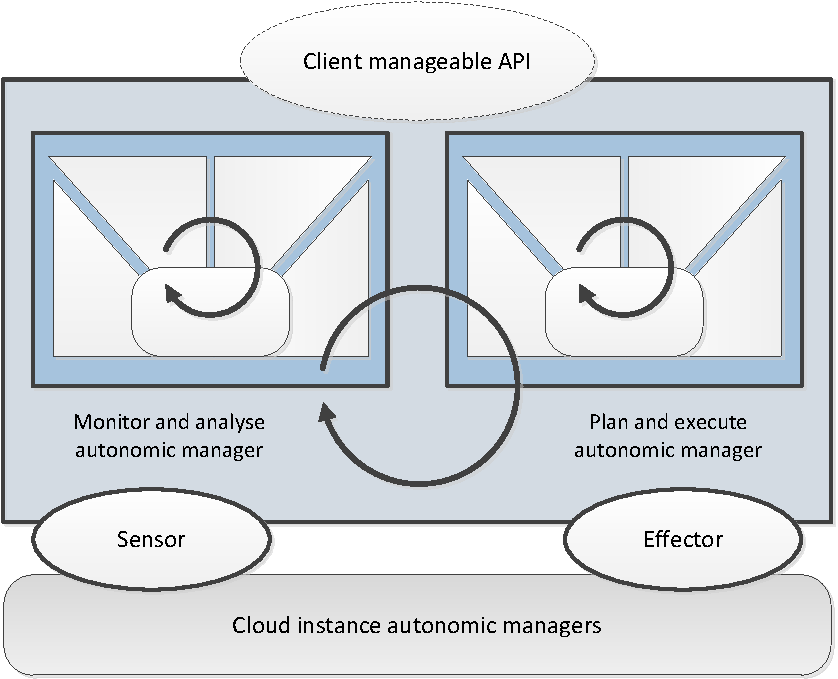
\includegraphics[width=0.7\textwidth]{chapter-design/csap-orchestrating-autonomic-manager}
  \end{center}
  \caption{Design of an orchestrating autonomic manager}
  \label{img:orchestrating-autonomic-manager}
\end{figure}

\subsection{Managed resource}
As it was stated in the previous sections and can be seen in figure \ref{img:orchestrating-autonomic-manager}, \emph{cloud instance autonomic managers} are managed resources of this manager. Each cloud instance is a deployment environment for a service or a stack, i.e. it is possible to span the service across different clouds by deploying stacks which make up the given service to different providers. Of course it is legitimate to deploy the whole service to only one provider.
\subsubsection*{Touchpoints}
As the cloud federation manager has to gain information about the state of a given cloud instance and be able to order the deployment of a stack or a service, the cloud instance exposes its manageability interface and its two types:
\begin{asparaenum}
\item[\textbf{Sensors}] -- set of attributes which forms the state of a given cloud instance. Attributes should include inter alia overall resources usage, pricing, geographical location. The more thorough elaboration will be held in the section devoted to \emph{plan and execution manager}.
\item[\textbf{Effectors}] -- set of stack/service management operations, such as deploy, migrate or delete.
\end{asparaenum}

\subsection{Plan and Execution Autonomic Manager}
The main purpose of this component is to select, based on knowledge provided directly to this manager from \emph{monitor and analyze manager} or a user (i.e. the specification of a service), cloud providers for a given service and carry out the planned action. In the following sections a detailed description of each function is given.

\subsubsection{Plan}
The aim of this function is to give a detailed plan for the action to be performed. In the context of this dissertation the first output produced by this component, regarding the use cases of deploying a service and dynamically scaling it, is a \emph{service deployment plan}, which is a mapping between available resources (cloud instances in this case) and concrete stacks making up the service. The second, definitely less complex, is a queries scheme about the state of the already-deployed services which is based on user's requests. In this case the component only propagates the request to the execute function. As this is only a mediation, there will be no further elaboration on this aspect.

\begin{asparaenum}
  \item[\textbf{Problem description}]
The problem of resource management in cloud computing environments is hard and complex. This is because of several aspects, but we will highlight only two reasons. 

The first one is the characteristic of resources available in a cloud -- not only are they geographically distributed, but they can be under different administrative domains and can vary in accessibility. This places a heavy burden on cooperation possibilities across cloud providers, both in a technical and non-technical way as providers need to maintain the high level of trust in order to effectively  deliver its products. Additionally, different entities forms the resources -- starting from individual devices, through virtual machines and whole workstations, ending with clusters and data centers.

The second one are the increasing Quality-of-Service requirements from the clients. They want resources they use to be reliable, flexible (able to scale according to workload), fault-tolerant, energy-efficient and, of course, cheap. It is clear that clients and cloud vendors have different objectives and supply-and-demand patterns.

There are two main approaches to tackle the problem of effective resource management and scheduling:
  \begin{itemize}
    \item \textbf{conventional style}, in which the mapping decision is determined by some \emph{cost function}. The downside of this method is the fact that in many cases the decision is a function of system-centric parameters \cite{buyya2002economic} and because of it the outcome may lead to better utilization of cloud resources, not necessarily the user's application. What is more, this model treats all resources as if their cost was the same and applications are considered equally important what not always is the case. 

      The positive side of this method is the fact that it involves only one entity that governs the scheduling and allocating the resources. What is more, it is up to the platform how many factors should be incorporated in such a function. Depending on the needs, a more sophisticated or simpler matching algorithm be applied, e.g. an algorithm that takes into account only available budget of a client.
      
      Legion \cite{chapin1999legion} can be an example of a solution which uses this method.
    \item \textbf{economics-paradigm based} \cite{buyya2001case}, in which the decision is not made statically by one entity, but is driven by the users' requirements. The model tries to adopt the real-world economic solution that involves markets and brokers on the computational ground. In this paradigm, clients (representing \emph{demand}) want to solve their problems at the lowest possible price while assuring required Quality-of-Service requirements and constraints, such as time frame. Resource providers (representing \emph{supply}) want to maximise the utilization of their resources while keeping their prices at the level that is attractive for other customers.
      
      Here are the most common economic models which can be applied to resource scheduling and management \cite{buyya2002economic}:
      \begin{itemize}
        \item the commodity market model;
        \item the posted price model;
        \item the bargaining model;
        \item the tendering/contract-net model;
        \item the auction model;
        \item the bid-based proportional resource sharing model;
        \item the community/coalition/bartering model;
        \item the monopoly and oligopoly
      \end{itemize}
  \end{itemize}

\item[\textbf{Function input}] Depending on the actual request, this function can have access to different knowledge that makes its input:

  \begin{asparaenum}
  \item[\textbf{Service deployment}] When the user wants to deploy a service on a cloud infrastructure, they have to prepare its detailed description containing technical (stacks) and Quality-of-Service requirements. Additionally, this component should have access to shared knowledge regarding the information about every cloud instance that forms the federation. This should include resource capacity and utilization rates.
  \item[\textbf{Service scaling}] When an application needs to be scaled, there is available additional knowledge that this component should use of -- detailed information about service's performance up to that point, e.g. service resource utilization level (CPU, I/O), response time, its users profile including their geographical location and so on. This knowledge in a form of a prediction model should be passed to the component by the \emph{analyse} function.
  \end{asparaenum}

\item[\textbf{Function output}] As it was stated in the introductory section, this function produces \emph{service deployment plan}. In the same section we conducted a quick survey of the most common approaches to the resource allocation and mapping problem. The proposed architecture places no restrictions on the chosen approach, as both paradigms can be fitted into it. In the case of \emph{conventional approach}, this component should be equipped with a matching function that takes as an input service description (and the information of its so far execution in the case of an auto-scaling action), offers from cloud providers and make a final decision based on these arguments.
  In the other case, this component can be thought of a cloud exchange \cite{InterCloud10}, that brings together service producers and consumers. Autonomic cloud instance managers could be considered bid-makers and would compete with one another for the client. What is more, if the model is bid-based, the client can have implemented behaviour that would also allow them to participate in auctions. This could be done by introducing another component that would act in user's name.
\end{asparaenum}

\subsubsection{Execute}
This function takes either a query about the state of a service or a deployment plan of the given service and passes execution requests to the proper cloud instance autonomic managers.

\subsection{Monitor and Analyse Autonomic Manager}
\subsubsection*{Introduction}
In many cases designers of applications cannot in advance foresee the detailed requirements of resources of their products, e.g. the number of virtual machines comprising it. This is especially true in case of \emph{start-ups} when it is not known whether the product will catch public attention and who exactly matches the target audience. In such circumstances the cloud provider should be able to quickly adapt to new conditions to prevent the service from being unable to work properly, e.g. take into account the geographical location of the application's users and deploy a service in close proximity to them so as to minimize the latency.

As it was discussed in earlier chapters, the above-mentioned use case refers to \emph{scaling} capabilities of a cloud provider. However, even if a cloud provider has \emph{auto-scaling} mechanisms, there can be unacceptable delays in application response time because of the \emph{reactive} nature of the feature -- the system decides to scale the application based on the \emph{current} resource consumption and utilization rate. Since it involves instantiating and provisioning virtual machines there is always a time overhead associated with it. Hence, there is a need that a system could \emph{predict} demands and behaviours of a hosted service in a \emph{proactive} way. 

The goal of this component is to gather data about current performance of a deployed service and based on it perform an in-depth analysis which results in a resource usage prediction model and auto-scaling schemes. This is the objective of the \emph{monitor} and \emph{analyse} functions, respectively.

\subsubsection*{Prediction models}
One way to divide prediction models into categories is to classify each one as a \emph{reactive} or a \emph{proactive} one. Since in the introductory section there were given reasons why the reactive approach is inefficient, here is a short overview of proactive approaches to the issue.

Using pattern-matching algorithms is one method to tackle the problem and this approach was presented in \cite{caron2010forecasting}. In their work, the algorithm analyses past usage data of an application and tries to identify the most similar patterns to current resource usage characteristics by using a pattern-matching algorithm. Then the obtained patterns are interpolated and the final prediction model is evaluated.

A performance prediction model and only its statistical evaluation is presented in \cite{islam2012empirical}. In that work, the usage of two machine-learning algorithms, \emph{Error Correction Neural Network} and \emph{Linear Regression}, is proposed. Additionally, the authors analyse the problem from an application's provider point of view contrary to most of the work in the field.

An analysis regarding the effectiveness of usage a proactive approach rather than static allocation methods can be found in \cite{kupferman2009scaling}, where a set of scoring metrics is proposed as an efficiency evaluator.

\subsubsection{Monitor}
The main goal of this function is to collect all data regarding usage, performance, resource utilization, capacity and availability of every cloud instance that forms a federation. Further elaboration on the function can be done by aligning use cases of this component:
\begin{asparaenum}
\item[\textbf{Deployment of a new service}] When a new service is about to be deployed on a cloud federation, the system has to a priori aggregate information about resource capacity, utilization rates, geographical location and so on from cloud providers to be able to perform the best match of a cloud provider with the given service. This component should collect this information and make it available to other components by placing it in \emph{shared knowledge}.
  \item[\textbf{Scaling of a deployed service}] When a service which had been hosted on a cloud needs to be scaled, the similar knowledge as in the previous case is required to be passed to \emph{analyse} function to perform the perfect match of a cloud instance.
\end{asparaenum}

The knowledge that the component obtains is about current \emph{topology} (which cloud instances make the cloud federation, what is their geographical location, how are they related, etc.) and \emph{policies} (data required to be compared against policies of deployed serviced). What is more, for the system to be able to perform auto-scaling, the gathered information can be classified as \emph{problem determination knowledge} \cite{IBM06}.

We do not strive to list the data which is required to be collected by this component in a system that tries to conform to the proposed architecture as it completely depends on the system needs. We want to give an overview of possibilities instead and leave the decision to the implementers. The same applies to the components and technology of a persistence layer.

\subsubsection{Analyse}
This function takes knowledge about the cloud federation and a service as an input and outputs a \emph{prediction plan}, which should be helpful in choosing the cloud instance for an application.

In the introductory section a brief overview of some possible techniques and algorithms that can be used in the analyse component was presented. We do not impose a particular method on this component -- it is up to the system complexity and design, which solution would be more suitable to the given needs.

\section{Summary}
Cloud-SAP fills the gap in existing platforms by providing a standardised approach to scaling applications using a fine-grained actions and operating on different platform levels: starting from an execution environment and ending on a cloud federation. It is based on a concept of an autonomic system, providing methodical but flexible foundation for its implementation. What is more, Cloud-SAP leverages core benefits of such a system: promise of a self-configuration, self-optimisation, self-health, self-protection. It is driven by a customer-defined policies and consequently ensures that customer is served with demanded Quality-of-Service and optimised costs.


\chapter{Implementation}

\chapterintro{
  This chapter details a proof-of-concept implementation of Cloud-SAP architecture.
}

\section{Introduction}
Previous chapters detailed requirements that a self-manageable platform oriented toward Quality-of-Service assurance should comply with. Beside this, reference architecture known as Cloud-SAP was introduced. This chapter in turn highlights key elements of a proof-of-concept implementation of Cloud-SAP. Noticeably, our implementation is by all means not exhaustive and merely intends to prove that presented architecture successfully tackles raised challenges. Hence, we implemented only following subset of managers specified by Cloud-SAP:
\begin{itemize}
  \item Autonomic container manager
  \item Autonomic stack manager
  \item Autonomic cloud instance manager
  \item Autonomic cloud federation manager
\end{itemize}

Apart from that, we implemented minimal viable modules that is monitoring, analysis, planning and execution. For example, we based analysis solely on threshold model, discarding more advanced techniques that uses prediction mechanisms.

\section{Overview}
As previous section indicates, key elements of discussed implementation are as follows: autonomic container manager, autonomic stack manager, autonomic cloud instance manager, autonomic cloud federation manager. Taking their role in service deployment into account, we grouped them into auto-scaling and cloud brokerage subsystems. High level overview of system, including its internal and external elements is depicted in figure \ref{fig:hlo-implementation}. Diagram \ref{fig:csap-layers-subsystem} illustrates thee relationship between Cloud-SAP managers and above-mentioned subsystems. 

\begin{figure}[!ht]
  \begin{center}
    \includegraphics[width=\textwidth]{chapter-implementation/hlo-implementation}
  \end{center}
  \caption{High level system overview}
  \label{fig:hlo-implementation}
\end{figure}

\begin{figure}[!ht]
  \begin{center}
    \includegraphics{chapter-implementation/csap-layers-subsystem}
  \end{center}
  \caption{System parts and their relation with autonomic managers}
  \label{fig:csap-layers-subsystem}
\end{figure}

As one can see, our implementation is composed by following parts:
\begin{asparaenum}
 \item[\textbf{Auto-scaling subsystem}] Auto-scaling subsystem supervises service's life cycle, monitoring it and enacting scaling actions when necessary. It is concentrated on all service's aspects: containers, stacks and application instances thus it is in fact a group of autonomic managers composed by container, stack and cloud instance managers.

 \item[\textbf{Cloud brokerage subsystem}] Brokerage subsystem groups components that together mediates between cloud providers. In particular, it consists of:
  \begin{itemize}
   \item Cloud broker - probes cloud providers and selects best offer according to a given policy. In Cloud-SAP model, it plays a role of orchestrating autonomic manager, that is, autonomic cloud federation manager.
   \item Cloud client - delegates service provisioning request to a cloud broker.
  \end{itemize}
 
 \item[\textbf{Cloud provider}] External system that manages a group of resource such as computing nodes, storage and networking typologies. Particularly, it is able to deploy, shutdown, migrate and monitor containers. Although Cloud-SAP is utterly cloud provider independent, our implementation is solely focused on OpenNebula that uses OpenVZ as a hypervisor. We selected OpenNebula due to its simplicity, flexibility and our expertise in managing it. Choosing hypervisor, we were compelled to select one that is based on lightweight containers due to theirs flexibility in scaling as previously advocated. OpenVZ was a natural choice due to its maturity and our familiarity within it.
 
 \item[\textbf{Application provider}] An entity that is interested in application scaling and deployment. It can be represented by a human being as well as by an external system.
\end{asparaenum}

With those information in mind, we can illustrate overall architecture, components and communication protocols on deployment diagram \ref{fig:hlo-deployment}. Successive sections portrays in detail specified elements.

\begin{figure}[!ht]
  \begin{center}
    \includegraphics{chapter-implementation/hlo-deployment}
  \end{center}
  \caption{Deployment diagram of a Cloud-SAP implementation}
  \label{fig:hlo-deployment}
\end{figure}


\section{Auto-scaling subsystem}

\begin{figure}[!ht]
  \begin{center}
    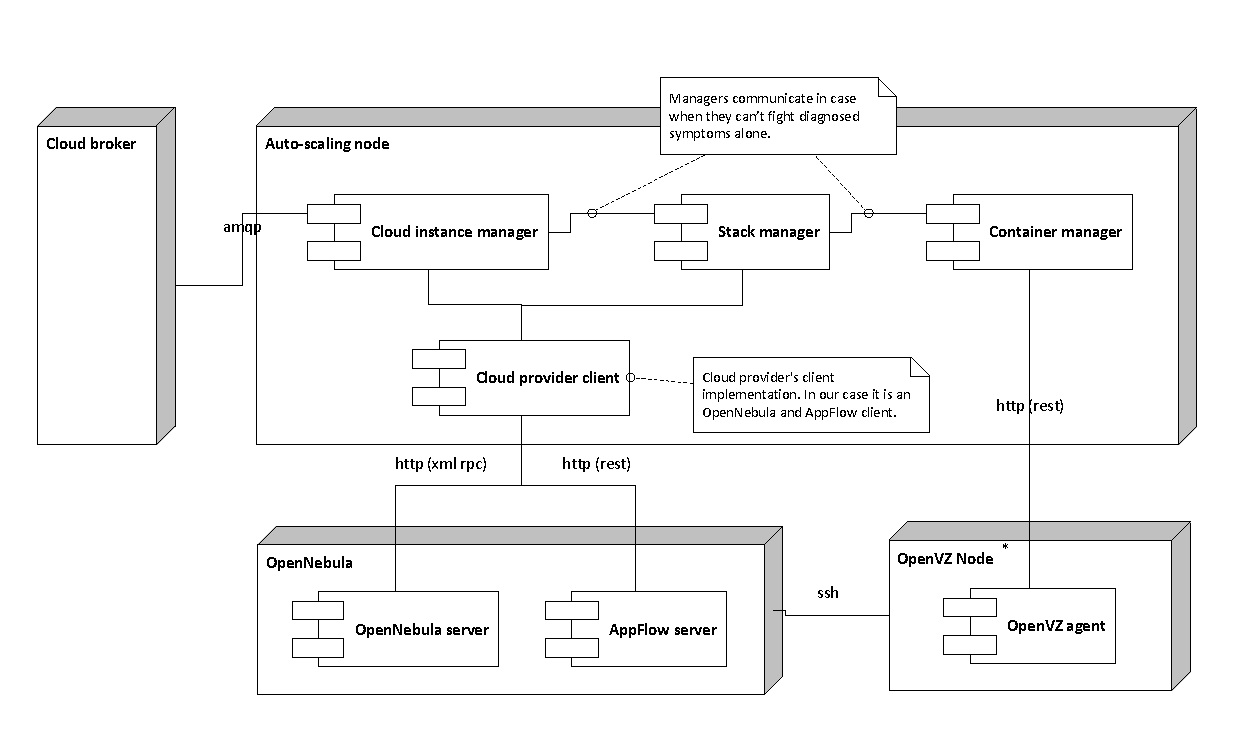
\includegraphics[width=\textwidth]{chapter-implementation/auto-scaling-subsystem-deployment}
  \end{center}
  \caption{Deployment diagram of a auto-scaling subsystem}
  \label{fig:auto-scaling-subsystem-deployment}
\end{figure}

\section{Cloud brokerage subsystem}

\section{Cloud provider}

\section{Exemplary scenarios}

\subsection{Service deployment}

\subsection{Scaling application}

\subsection{Scaling application across multiple cloud providers}

\section{Summary}


\chapter{Evaluation}

\chapterintro{
  This chapter contains results and discussions on the evaluation of tests run on the proposed solution.
}

\section{Introduction}
We carried out a number of tests which aim to prove the solution to be better than currently available, especially in terms of:
\begin{enumerate}
  \item deployment cost
  \item cost of providing given Quality-of-Service
  \item deployment time
\end{enumerate}

\subsection*{Hardware and virtual machines configuration}
All tests that were carried out were run on the same hardware and/or used the same virtual machines as presented in table \ref{tab:test-deployment-time-common-hardware-configuration}.

\begin{table}
  \centering
  \begin{tabular}{ l l l l l }
    \specialrule{.1em}{.05em}{.05em}                  
    \textbf{Name} & \textbf{VM} & \textbf{CPU} & \textbf{RAM} & \textbf{HD} \\
    \specialrule{.1em}{.05em}{.05em} 
     Desktop   &    & Intel(R) Core(TM) i5-2500 CPU @ 3.30GHz & 8GB & 1TB \\ \hline
     Node1   &     & AMD Athlon\texttrademark 64 X2 Dual Core, 2000MHz & 3GB & 160GB \\ \hline
     Node3  &      & AMD Sempron(tm) Processor 3000+ & 2.5GB & 160GB \\ \hline
     Node4  &      & AMD Duron(tm) Processor 1GHz& 2.5GB & 60GB \\ \hline
     Frontend\{1,2\} & \checkmark & 1 CPU & 512MB & 10GB \\
    \hline  
  \end{tabular}
  \caption{Configuration of hardware/virtual machines used during tests}
  \label{tab:test-deployment-time-common-hardware-configuration}
\end{table}

\section{Cost of service deployment}
\subsection*{Description}
The aim of this test case is to test the primary use case of the proposed solution -- deployment of a service with the emphasis on client's \textbf{cost}. It should show that the platform chooses the best mapping between the stacks and cloud providers so that the client's pays the \textbf{lowest} possible price.

\subsection*{Preconditions}
Service specification (\ref{lst:service-spec-test-cost}) forms an input to the application. Its elements are different software stacks that are parts of the whole service. Each cloud provider has its own price for a given software stack which is shown in table \ref{tab:test-service-deployment-cost}. Diagram \ref{fig:deployment-cost-physical-nodes} illustrates the simplified environment setup.

\begin{table}
  \centering
  \begin{tabular}{ c  c  c  c  }
    \specialrule{.1em}{.05em}{.05em}                  
    & \textbf{CP-1} & \textbf{CP-2} & \textbf{CP-3} \\
    \specialrule{.1em}{.05em}{.05em}                  
    java      & 150 & 120 & 180 \\ \hline
    ruby      & 220 & 290 & 250 \\ \hline
    postgres  & 320 & 240 & 290 \\ \hline
    python    & 200 & 260 & 180 \\ \hline
    amqp      & 330 & 390 & 285 \\
    \hline  
  \end{tabular}
  \caption{Price for a stack in the given cloud provider}
  \label{tab:test-service-deployment-cost}
\end{table}

\begin{figure}[!ht]
  \begin{center}
    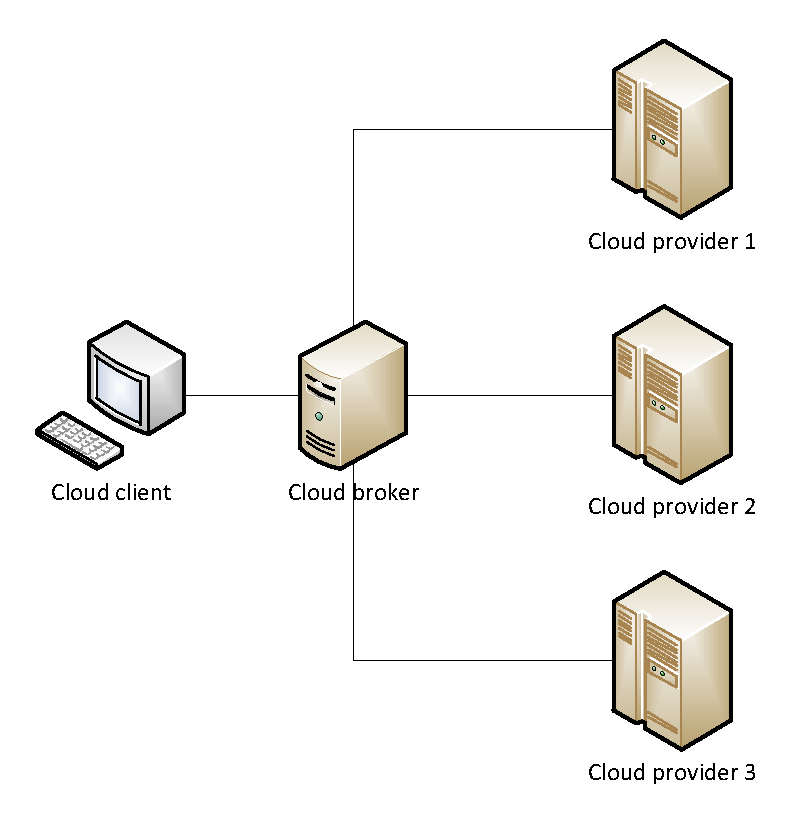
\includegraphics[width=0.6\textwidth]{chapter-evaluation/deployment-cost-physical-nodes}
  \end{center}
  \caption{Deployment cost: environment configuration}
  \label{fig:deployment-cost-physical-nodes}
\end{figure}


\subsection*{Results}
Table \ref{tab:test-service-deployment-cost-mapping} shows obtained mapping between stacks and cloud providers. Taking into account this result, figure \ref{ch7:service-deployment-cost} shows comparison of cost the client would have to pay with and without such a mapping.

\begin{table}
  \centering
  \begin{tabular}{ c c c  c  }
    \specialrule{.1em}{.05em}{.05em}                  
    & \textbf{CP-1} & \textbf{CP-2} & \textbf{CP-3} \\
    \specialrule{.1em}{.05em}{.05em}                  
    java      & & x & \\ \hline
    ruby      & x & & \\ \hline
    postgres  & & x & \\ \hline
    python    & & & x \\ \hline
    amqp      & & & x \\
    \hline  
  \end{tabular}
  \caption{Chosen cloud providers for the given stack}
  \label{tab:test-service-deployment-cost-mapping}
\end{table}

\begin{figure}[!ht]
  \begin{center}
    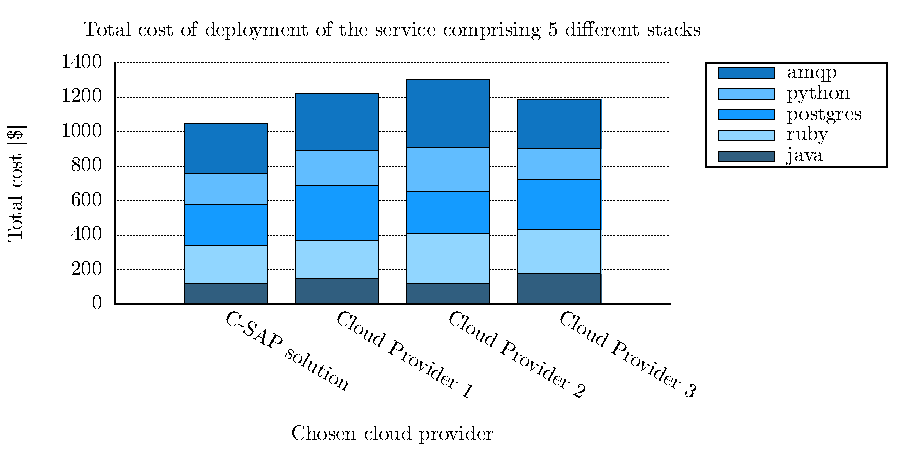
\includegraphics{chapter-evaluation/case-study-service-deployment-reduced-client-costs}
  \end{center}
  \caption{Comparison of the deployment cost when the service is deployed only on a selected cloud provider or a combination of cloud providers selected by Cloud-SAP}
  \label{ch7:service-deployment-cost}
\end{figure}

\newpage
\subsection*{Conclusion}
Obtained results clearly show that our proof-of-concept product met expectations of this test case as the client was offered the cheapest deployment scheme among various cloud providers for a given software stack.
The mapping mechanism is simple yet considerably powerful -- in this simple scenario the savings were significant since they constituted nearly 20 percent of the price offered by \emph{Cloud Provider 2}. This shows that implementing similar solutions in the real world could be of great benefit to cloud consumers.

\newpage
\section{Auto-scaling -- single-provider based}
\subsection*{Description}
\begin{asparaenum}
\item[\textbf{Motivation}]The aim of this test-case is to show that introducing a multi-layered auto-scaling platform is of a great benefit in terms of cost and resource usage for cloud consumers and cloud providers respectively. What is more, this test should prove that once there are many levels on which scaling operations can be performed, there are significant reduction in costs paid by consumers.
We want to prove it by comparing our proof-of-concept product to \emph{Carina} \cite{Carina}. \emph{Carina} embraces a whole range of various scaling policies for users' environments (environment, in this context, means an application with all its software dependencies that are to be deployed on the cloud), but there is only one way in which they are executed -- by managing the number of virtual machines (i.e. horizontal scaling). Quite on the contrary, \emph{Cloud-SAP} has mechanisms that allow to scale the environment vertically in the first place and if that turns out to be not sufficient, horizontally. This test shows the influence of lack/presence of this feature on price and resource consumption.
\item[\textbf{Scenario}] The test scenario involves
  \begin{inparaenum}[a)]
    \item deployment of a sample environment on the cloud,
    \item substitute the real module responsible for collecting CPU usage date for a mock one,
    \item monitoring the scaling actions performed by each solution,
    \item evaluation of the cost the client has to pay for the service.
  \end{inparaenum}
  Deployment of a service is done in a product-specific manner (up to the point where the vm deployment request is passed to OpenNebula). Mocking the CPU usage was possible by replacing the part in \emph{InformationManager} responsible the collecting CPU data in a host for a request to a web service which generated a time-based mocked-values. Choosing the appropriate function is another issue and is discussed in the next paragraph.
\end{asparaenum}

\subsubsection*{CPU usage function}
We wanted to ensure that both solutions, \emph{Carina} and \emph{Cloud-SAP}, collected the same data regarding the CPU usage for the given time. What is more, the curve should resemble CPU usage in the real business scenarios as much as possible. Thus, we took into account the following factors:
\begin{itemize}
  \item every peak in CPU usage should be followed by a gradual descent which would mimic the real auto-scaling actions executed by each solution,
  \item (boundary conditions) CPU usage should be between 0 and 100 and, additionally, should exceed the previously set scaling threshold value of each solutions so that it would trigger the scaling policies evaluation
  \item once the scaling operations have completed, CPU usage should be constant at a rate which would not introduce any changes in the environment settings (such as the number of virtual machines and parameters of any virtual machine)
\end{itemize}
To find the equation of a function that would satisfy the previously-mentioned requirements we used \emph{polynomial interpolation}. As we chose 4 points which were the input to the algorithm, we got a cubic polynomial as an output. Adding further constraints to mimic two spikes in CPU usage resulted in the function whose formula is in \eqref{eq:cpu-mock-usage} and plot in figure \ref{fig:auto-scaling-1cp-cpu-usage-function}.
\begin{eqnarray}
  %f(x) = (1751 *x)/132+(3 *x**2)/8-(31* x**3)/264
  %x <= 11.583 ? f(x) : ( x <= 21.441 ?  f(x - 10) : 25 )
  f(x) &=& -\frac{31}{264}x^3+\frac{3}{8}x^2+\frac{1751}{132}x \nonumber \\
  CPU\_usage(t) &=& \left\{
  \begin{array}{l l l}
    f(t) & \quad 0 & \le t < 11.583 \\
    f(t-10) & \quad 11.583 & \le t < 21.441 \\
    25 & \quad 21.441 & \le  t \\
\end{array} \right.
\label{eq:cpu-mock-usage}
\end{eqnarray}

\begin{figure}[!ht]
  \begin{center}
    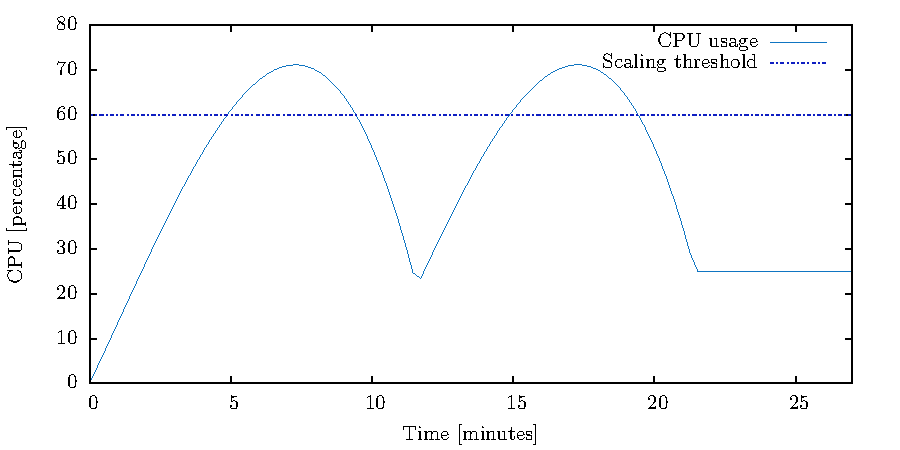
\includegraphics{chapter-evaluation/cpu-usage-mock}
  \end{center}
  \caption{Auto-scaling - single-provider based: CPU usage function}
  \label{fig:auto-scaling-1cp-cpu-usage-function}
\end{figure}

Because \emph{Carina} is capable of only horizontal scaling and \emph{Cloud-SAP} of both horizontal and vertical, one can question whether the descent in CPU usage can be actually the same in both cases. To answer this question we want to look into the description of the virtual machines comprising the deployed environment. It states that each VM can use up to 30\% power of a single host's CPU. Thus, we can be fairly sure that adding another virtual machine that uses 0.3 CPU capacity of its host is equivalent with changing the CPU usage settings of already deployed VM from 30 to 60\%.
\subsection*{Preconditions}
\subsubsection*{Environment specification}
\begin{asparaenum}
  \item[\textbf{Auto-scaling policy specifications}] As it is shown in figure \ref{fig:auto-scaling-1cp-cpu-usage-function}, we set in both products the threshold values of CPU usage that trigger performing auto-scaling actions to 20 and 60 percent. To apply this setting, the auto-scaling part of service specification looks as follows: in Carina the user has to add the parameters of an auto-scaling policy in a hash that describes the environment under key \emph{:elasticy\_policy}. It is possible to specify the minimal and the maximal number of virtual machines that forms the environment and, what is most important, expressions whose evaluation results in scaling the application. The part responsible for this is shown in listing \ref{lst:auto-scaling-1cp-carina-service-spec}.\lstinputlisting[caption=Carina service specification used for testing auto-scaling with 1 cloud provider, label=lst:auto-scaling-1cp-carina-service-spec]{auto-scaling-1cp-carina-service-spec} In Cloud-SAP it is a matter of setting appropriate arguments to a specific policy. In this case the policy is \emph{threshold\_model} and values are 20 and 60 for lower and upper bound respectively. The auto-scaling part from service specification is shown in listing \ref{lst:auto-scaling-1cp-cloud-sap-service-spec}. \lstinputlisting[caption=Cloud-SAP service specification used for testing auto-scaling with 1 cloud provider, label=lst:auto-scaling-1cp-cloud-sap-service-spec]{auto-scaling-1cp-cloud-sap-service-spec}
  \item[\textbf{OpenNebula/Carina/Cloud-SAP configuration}] Since Carina and Cloud-SAP used two different instances of OpenNebula installed on separate virtual machines, it is essential the configuration be the same on each of them. Listing \ref{lst:auto-scaling-1cp-one-config} shows the most important OpenNebula excerpt from settings file used in this test case -- polling interval specification, which was set to 30 seconds. To ensure that both products can actually use up-to-date data, they should figure their policies every 30 seconds or longer. In Carina the user cannot specify this value, because it is hard-coded in source code to 60 seconds. In Cloud-SAP, however, this value was set in a configuration file and was equal to 60 seconds as well as in Carina. \lstinputlisting[caption=OpenNebula configuration excerpt -- information manager, label=lst:auto-scaling-1cp-one-config]{auto-scaling-1cp-one-config}. Vertical scaling mechanism in \emph{Cloud-SAP} is implemented in a way that causes exponential growth of CPU resources consumption. When there is a need to perform a scaling action on CPU usage, current value is taken and increased by 30\%.
  \item[\textbf{Deployment diagrams}] Deployment diagrams show the placement of each component in both installations. They are shown in figures \ref{fig:auto-scaling-1cp-carina-deployment-diagram} and \ref{fig:auto-scaling-1cp-cloud-sap-deployment-diagram}.

  \begin{figure}[!ht]
    \begin{center}
      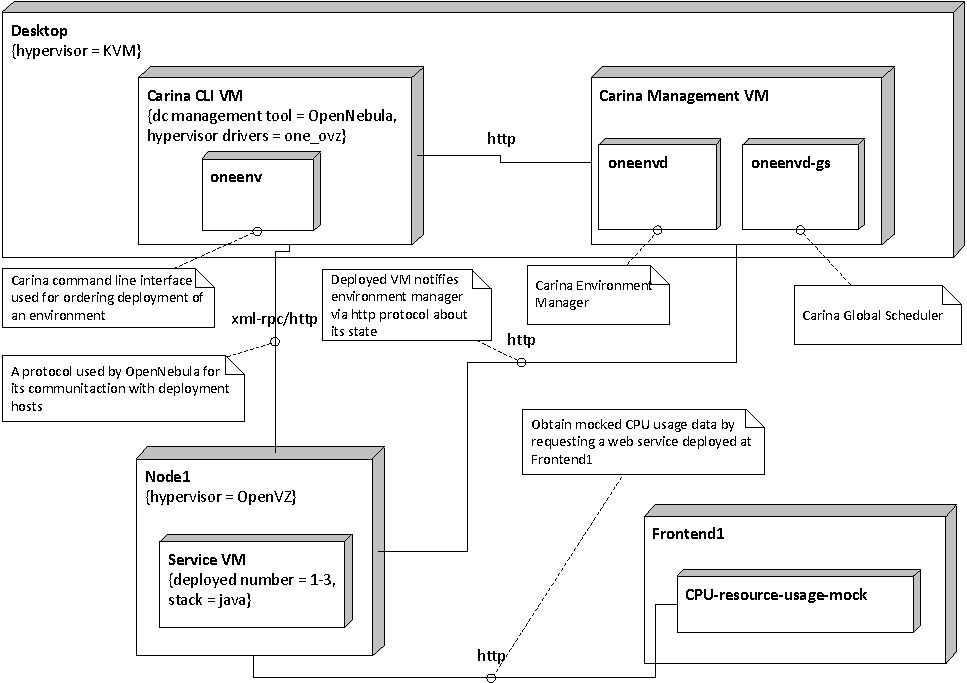
\includegraphics{chapter-evaluation/cpu-usage-carina-deployment-diagram}
    \end{center}
    \caption{Auto-scaling - single-provider based: deployment diagram of Carina}
    \label{fig:auto-scaling-1cp-carina-deployment-diagram}
  \end{figure}

  \begin{figure}[!ht]
    \begin{center}
      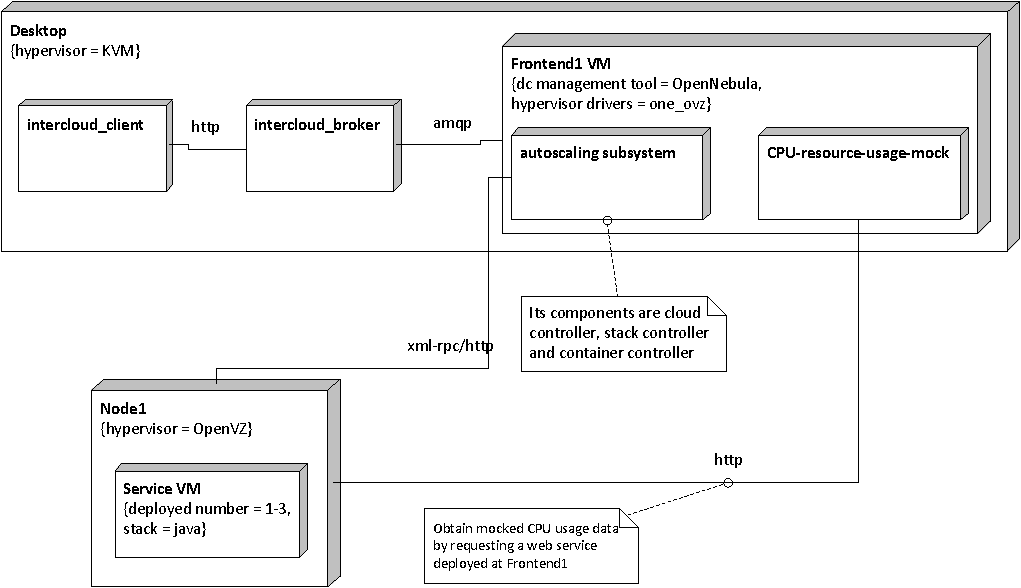
\includegraphics{chapter-evaluation/cpu-usage-cloud-sap-deployment-diagram}
    \end{center}
    \caption{Auto-scaling - single-provider based: deployment diagram of Cloud-SAP}
    \label{fig:auto-scaling-1cp-cloud-sap-deployment-diagram}
  \end{figure}

  \end{asparaenum}

\newpage
\subsubsection*{Hardware/VM configuration}
All virtual machines were deployed onto \emph{Node1}, which uses \emph{OpenVZ} as a virtualization technology and whose hardware configuration can be found in table \ref{tab:test-deployment-time-common-hardware-configuration}. \emph{OpenNebula} was installed on a \emph{Frontend1} virtual machine and its configuration is in the same table. \emph{Carina} required the usage of 2 virtual machines which were deployed on \emph{Desktop} with KVM as a hypervisor and whose configuration is in table \ref{tab:test-auto-scaling-1cp-hardware-configuration}. Diagram \ref{fig:auto-scaling-1cp-physical-nodes} illustrates the physical setup of the test-case. 

\subsubsection*{Test case duration}
The test case lasts 25 minutes as the CPU usage is constant and equals 25\% after 21 minutes and 44 seconds.

\begin{table}
  \centering
  \begin{tabular}{  l  l  l  l  }
    \specialrule{.1em}{.05em}{.05em} 
     
    \textbf{Name} & \textbf{CPU} & \textbf{RAM} & \textbf{HD} \\
    \specialrule{.1em}{.05em}{.05em} 

    (virtual machine) carina-frontend  & 1 CPU & 1GB & 6GB \\ \hline
    (virtual machine) carina-management-vm  & 1 CPU & 1GB & 9GB \\
    \hline  
  \end{tabular}
  \caption{Configuration of hardware/virtual machines used during tests}
  \label{tab:test-auto-scaling-1cp-hardware-configuration}
\end{table}

\begin{figure}[!ht]
  \begin{center}
    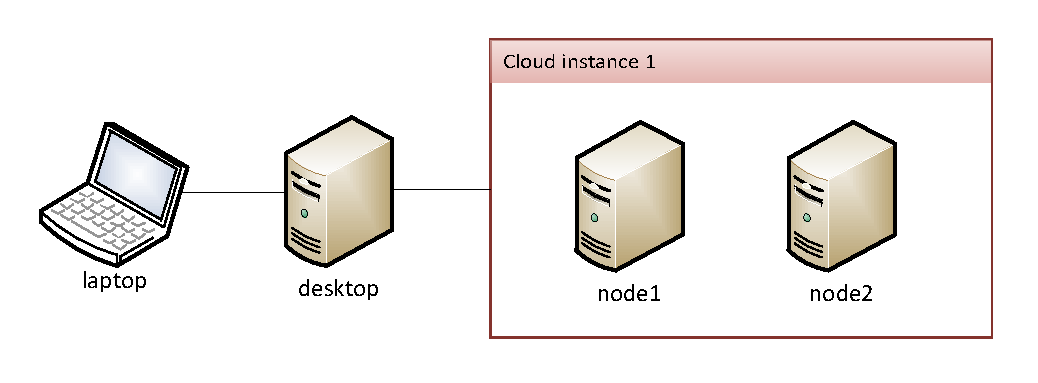
\includegraphics[width=0.8\textwidth]{chapter-evaluation/auto-scaling-1cp-physical-nodes}
  \end{center}
  \caption{Auto-scaling - single-provider based: environment configuration}
  \label{fig:auto-scaling-1cp-physical-nodes}
\end{figure}


\subsection*{Expectations}
As auto-scaling behaviour of both products is determined by CPU usage of the deployed service, we can predict the outcome of the test by thorough analysis of the plot in figure \ref{fig:auto-scaling-1cp-cpu-usage-function}.

The first conclusion is that all auto-scaling actions are performed after exceeding the upper threshold value of CPU usage, this is 60 percent in our case what happens about 5 minutes after the deployment of an environment is completed. CPU consumption remains high for about 2 minutes what enables both products to take appropriate, auto-scaling steps. We expect \emph{Carina} to deploy another virtual machine and \emph{Cloud-SAP} to scale vertically. Then it gradually goes down, which simulates that all taken actions have successfully completed. Then, after another several minutes, the cycle recurs, but this time we expect the proposed solution to scale horizontally. \emph{Carina} is expected to behave as in the previous cycle. Once the cycle has completed, after roughly 21 minutes, the value of CPU consumption remains constant at 25 percent and the test is completed.
\subsection*{Results}
  In the first place it is worth discussing the results of \emph{Carina} and \emph{Cloud-SAP} separately and then compare resource consumption of each solution and its influence on cost paid by the end-user.

\begin{asparaenum}

  \item[\textbf{Cloud-SAP}] Our proof-of-concept solution behaved exactly as expected. To make the discussion more clear, there is an excerpt from a log file of this test run in listing \ref{lst:auto-scaling-1cp-results-csap-logs}. \lstinputlisting[caption=Cloud-SAP logs excerpt regarding auto-scaling actions, label=lst:auto-scaling-1cp-results-csap-logs]{auto-scaling-1cp-results-csap-logs}


\item[\textbf{Carina}] As \emph{Carina} is capable only of horizontal scaling, in discussion of its resource usage we can confine ourselves to counting the number of deployed virtual machines in the given time intervals. In the log files we can trace all actions that were triggered during the test case. As listing \ref{lst:auto-scaling-1cp-results-carina-jobs} shows, they completely met the expectations expressed in the previous section -- there were two ''SCALEUP'' jobs which resulted in increase of the total number of virtual machines comprising the environment. The one-hour shift in the listing is caused by the wrong clock setting on a virtual machine.  \lstinputlisting[caption=Carina environment manager logs with taken actions (\emph{jobs}), label=lst:auto-scaling-1cp-results-carina-jobs]{auto-scaling-1cp-results-carina-jobs}
Since the base configuration assumed that the environment consists of 2 virtual machines, we can say that about 10 minutes after deployment of an environment, the number of VMs increased to 3, and after another 10 minutes, to 4.

Deployment finished at 15:25:45 and at this time we started the mock-cpu-usage web service. When the platform concluded that there are insufficient resources, it tried for three times changing parameters (virtual CPU used by the vm) of the virtual machines forming the service. Once scaling vertically was not possible such an information was passed to cloud controller which performed scaling across different cloud providers.
\end{asparaenum}

\subsubsection*{Cost}
In our scenario cost is roughly equivalent with the CPU usage, so the plot of a cost virtually presents the CPU usage. Figure \ref{fig:auto-scaling-1cp-cost-comparison} shows CPU usage by environment when deployed and configured by two competing products.
\begin{figure}[!ht]
  \begin{center}
    \includegraphics{chapter-evaluation/auto-scaling-1cp-cost-comparison}
  \end{center}
  \caption{Auto-scaling - single-provider based: comparison of cost/CPU usage}
  \label{fig:auto-scaling-1cp-cost-comparison}
\end{figure}
If we were to roughly estimate the cost in both solutions it would be equal in Carina:
\begin{equation}
  7\cdot 0.3 + 10\cdot 0.6 + 8\cdot 0.9 = 15.3 \quad \text{[currency unit]}
\end{equation}
and in Cloud-SAP:
\begin{equation}
  7.0166\cdot 0.3 + 2\cdot 0.39 + 2.01667\cdot0.507 + 7.05\cdot 0.659 + 6.91667\cdot 0.959 \approx 15.186483
\end{equation}

\subsection*{Conclusion}
The obtained results shows that the proposed solution has enormous potential in terms of better utilisation of available resources of the cloud and reducing cost paid by cloud consumers.

Judging by the plot of cost (figure \ref{fig:auto-scaling-1cp-cost-comparison}), we can be fairly sure that it is possible to obtain better results by proper tuning of the scaling vertical mechanism. In particular, one can consider changing the default CPU growth from 1.3 to other or apply a different strategy, for example a growth by a constant rate. What is more, in order to get the best results, the policy scaling interval must be chosen with a great care with the consideration of specific parameters of a given environment.

\newpage
\section{Auto-scaling -- multiple-provider based}
\subsection*{Description}

\subsubsection{Motivation} This test case aims to prove that scaling across multiple cloud providers is vitally important when ensuring appropriate Quality-of-Service, especially in cases of increased number of service requests. Such scaling scenario, known also as cloud-bursting, leverage benefits arising from offloading application load to an external provider. In order to verify our concept we compare number of transactions per second guaranteed by \emph{Cloud-SAP} and \emph{Carina}. While our proof of concept solution features multi-layer scaling and is cloud federation aware, \emph{Carina} adopts only horizontal scaling. It is expected that test case prove benefits emerging from enriching application platform provider with a cloud federation awareness.
 
\subsubsection{Scenario}
Testing requires following steps to be done:
\begin{enumerate}
\item deploy an exemplary service
\item observe system behaviour under load, simulated by a resource usage mock. It is vital for a resource usage to exceed a single provider capabilities
\item assess system characteristics, including number of handled transactions per second
\end{enumerate}

\subsubsection*{Load simulation}
Similarly to a previous test case, we leveraged a resource mock that allows us to precisely control monitoring information returned to an system. Besides, in order to simplify test case, we were solely focused on a CPU usage. CPU usage function has to exceed upper threshold limit at some point and stay at that level, triggering successive auto-scaling events. However, at some point single cloud provider resources will be surpassed. Equation \eqref{eq:cpu-mock-usage-2cp} denotes a resource usage function that is expected to fulfil above-mentioned conditions and is illustrated in figure \ref{fig:auto-scaling-2cp-cpu-usage-function}.
\begin{equation}
 f(x) = \frac{29}{1500}x^3-\frac{21}{20}x^2+\frac{533}{30}x
 \label{eq:cpu-mock-usage-2cp}
\end{equation}

\begin{figure}[!ht]
  \begin{center}
    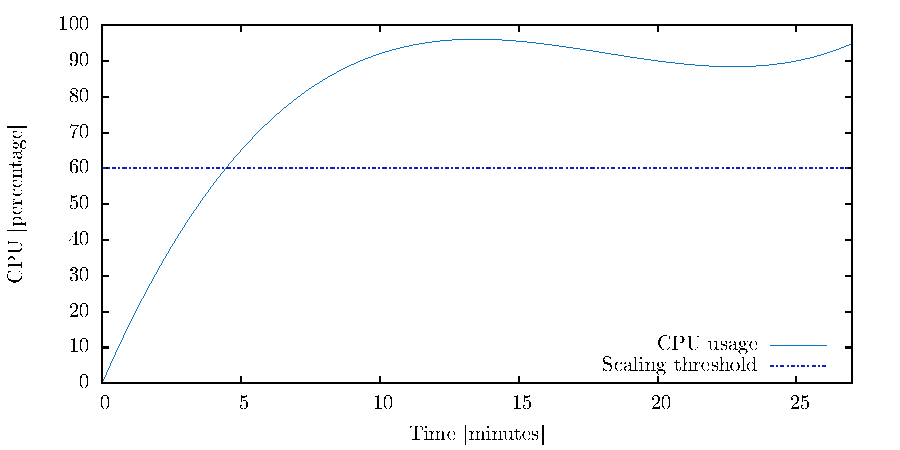
\includegraphics{chapter-evaluation/cpu-usage-mock-multiple}
  \end{center}
  \caption{Auto-scaling - multiple-provider based: CPU usage function}
  \label{fig:auto-scaling-2cp-cpu-usage-function}
\end{figure}


\subsection*{Preconditions}
\subsubsection*{Environment specification}
\begin{asparaenum}
  \item[\textbf{Auto-scaling policy specifications}] Policies used in this test are based on a threshold model with the following properties:
  \begin{itemize}
   \item value below 20 triggers scaling down event
   \item value grater than 60 triggers scaling up event
  \end{itemize}
  However, considering the fact that we are entirely focused on scaling up, only the upper limit is relevant in our case. Listings \ref{lst:auto-scaling-2cp-carina-service-spec} and \ref{lst:auto-scaling-2cp-cloud-sap-service-spec} presents scaling policies for \emph{Carina} and \emph{Cloud-SAP} respectively.
  
  \lstinputlisting[caption=\emph{Carina} service specification used for testing auto-scaling with 2 cloud providers, label=lst:auto-scaling-2cp-carina-service-spec]{auto-scaling-2cp-carina-service-spec}
  \lstinputlisting[caption=\emph{Cloud-SAP} service specification used for testing auto-scaling with 2 cloud providers, label=lst:auto-scaling-2cp-cloud-sap-service-spec]{auto-scaling-2cp-cloud-sap-service-spec}
  
  \item[\textbf{OpenNebula/Carina/Cloud-SAP configuration}] 
  Components common to \emph{Carina} and \emph{Cloud-SAP}, namely \emph{OpenNebula} instances and computing nodes, were configured in the same fashion. Listing \ref{lst:auto-scaling-2cp-one-config} depicts key configuration elements of \emph{OpenNebula} monitoring mechanism.
  
  \lstinputlisting[caption=OpenNebula configuration excerpt -- virtual machine and information manager, label=lst:auto-scaling-2cp-one-config]{auto-scaling-2cp-one-config}
  
  \item[\textbf{Deployment diagrams}] Components that took part during test are show in figures \ref{fig:autoscale-2cp-cloud-sap-deployment-diagram} and \ref{fig:auto-scaling-2cp-carina-deployment-diagram}.

  \begin{figure}[!ht]
    \begin{center}
      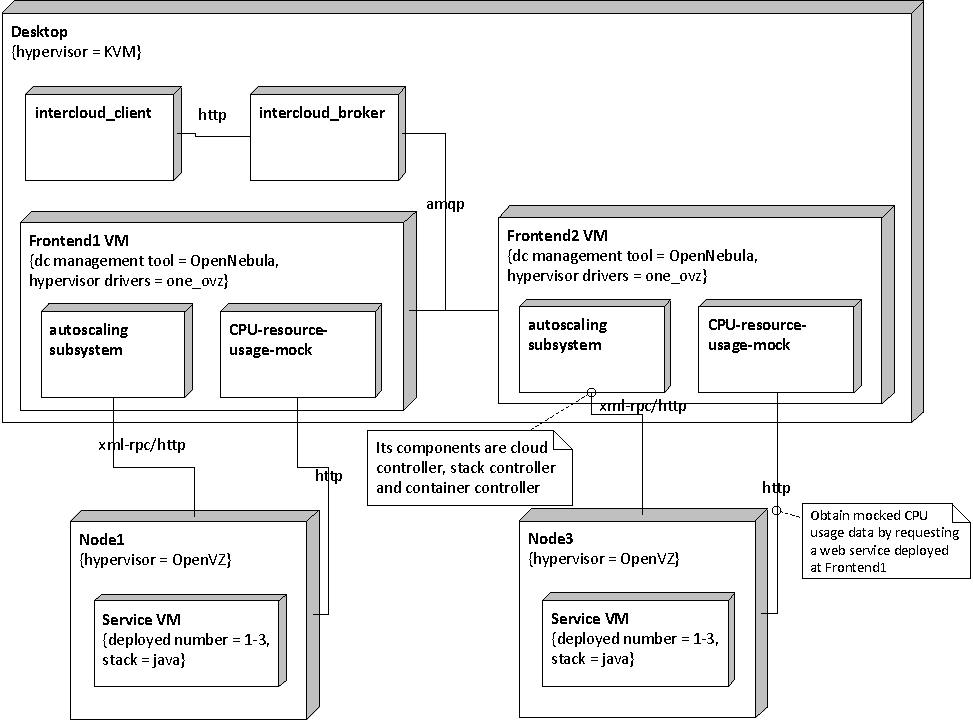
\includegraphics{chapter-evaluation/autoscale-2cp-cloud-sap-deployment-diagram}
    \end{center}
    \caption{Auto-scaling - multiple-provider based: deployment diagram of \emph{Cloud-SAP}}
    \label{fig:autoscale-2cp-cloud-sap-deployment-diagram}
  \end{figure}
  
  \begin{figure}[!ht]
    \begin{center}
      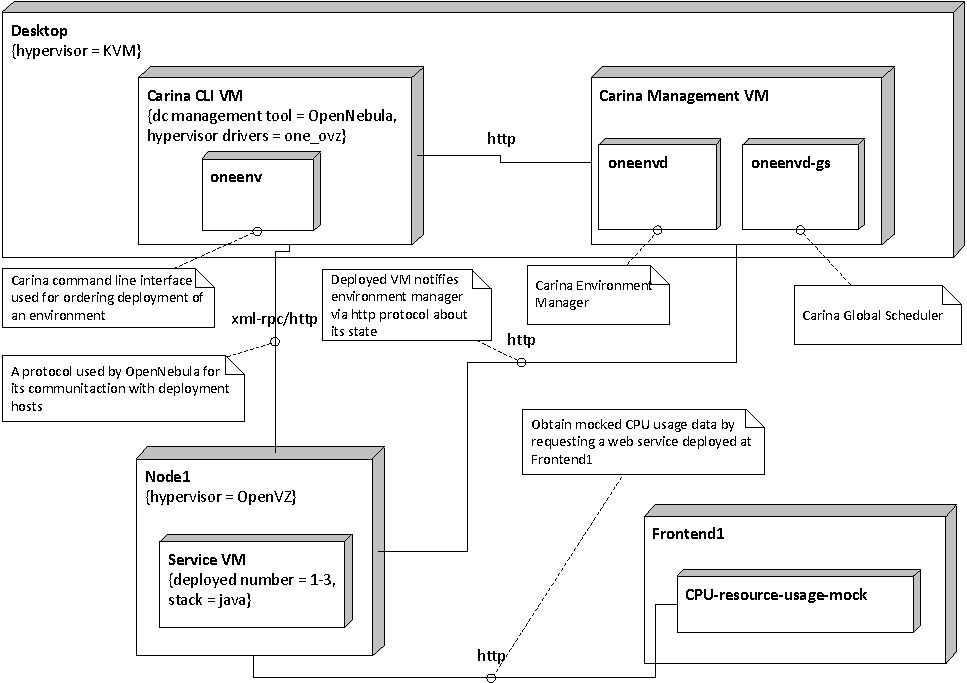
\includegraphics{chapter-evaluation/cpu-usage-carina-deployment-diagram}
    \end{center}
    \caption{Auto-scaling - multiple-provider based: deployment diagram of \emph{Carina}}
    \label{fig:auto-scaling-2cp-carina-deployment-diagram}
  \end{figure}
\end{asparaenum}

\subsubsection*{Hardware/VM configuration}

Figure \ref{fig:auto-scaling-2cp-physical-nodes} depicts physical configuration of the environment. In short, setup was as follows: all \emph{Cloud-SAP} components, apart from cloud client deployed on \emph{Laptop}, were provisioned on \emph{Desktop}. \emph{Cloud Proivder 1 (CP-1)} is \emph{OpenNebula} instance known as \emph{Frontend1} which uses \emph{Node1} as a computing node and is deployed on \emph{Desktop}, while \emph{CP\-2} uses \emph{Frontend2} and \emph{Node2}. Specification of nodes is listed in table: \ref{tab:test-deployment-time-common-hardware-configuration}. Deployment cost of a java stack was 50 and 60 using \emph{CP-1} and \emph{CP-2}, respectively.

\begin{figure}[!ht]
  \begin{center}
    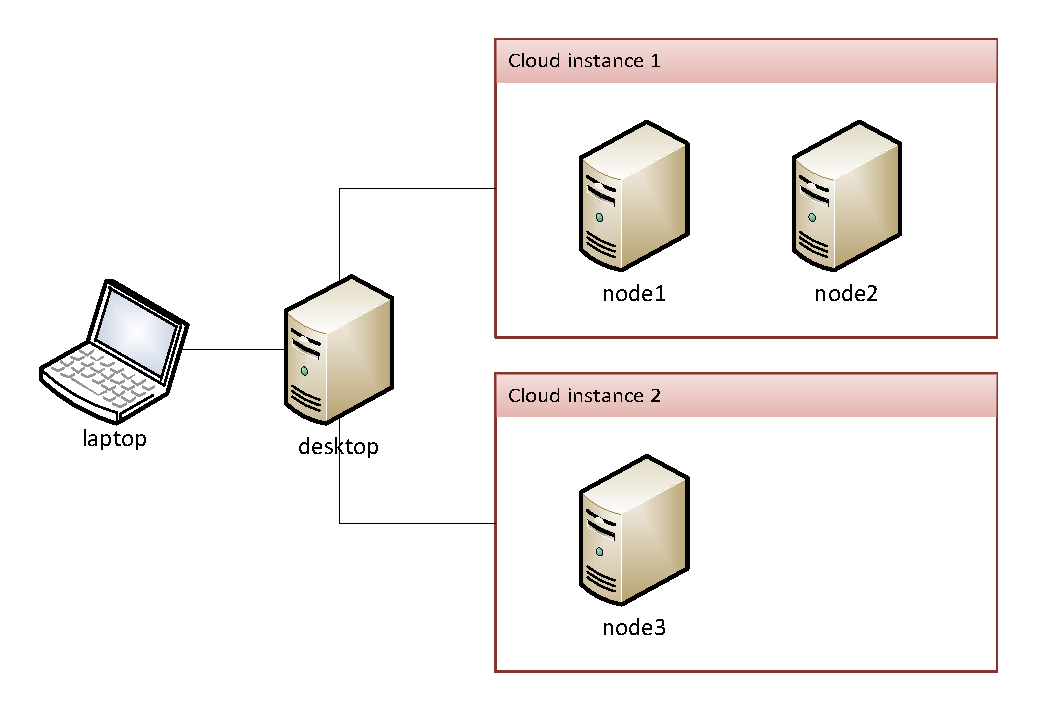
\includegraphics[width=0.85\textwidth]{chapter-evaluation/auto-scaling-2cp-physical-nodes}
  \end{center}
  \caption{Auto-scaling - multiple-provider based: environment configuration}
  \label{fig:auto-scaling-2cp-physical-nodes}
\end{figure}

\subsubsection*{Test case duration}
The test case lasts 25 minutes.


\newpage
\subsection*{Expectations}
Taking CPU usage function into account, we can predict outcome of the test. Scaling policy is violated in 5th minute, hence, it is expected that first scaling event occur after that point. Moreover, since that moment, CPU usage remains beyond threshold implying successive scaling actions.

Due to the fact that \emph{Cloud-SAP} favours fine-grained scaling actions such as vertical scaling, it is expected that these actions occur sooner than horizontal scaling. However, at some point \emph{CP-1} capacity won't be sufficient, hence, another stack instance (one master instance, two slaves) will be deployed on \emph{CP-2}. Subsequent scaling actions will take place solely on a \emph{CP-2} 2 and will involve further vertical scaling.

Carina, on the other hand, supports solely horizontal scaling using single cloud provider. On top of that, it is assumed that succeeding slaves instances will be added to a service up to the point where Cloud Provider won't have enough resources to proceed with further scaling requests.

\subsection*{Results}

\begin{asparaenum}
  \item[\textbf{Cloud-SAP}] 
   In total, there were 13 vertical and 2 horizontal scaling events. First action took place minute after first violation of scaling policy rule. Since then, slaves' CPU were successively increasing to the point were further scaling wasn't possible - 13th minute of the test. Therefore, \emph{Cloud-SAP} deployed two new slaves on \emph{CP-2}. Listing \ref{lst:auto-scaling-2cp-results-csap-logs} presents logs covering service lifecycle. \lstinputlisting[caption=Cloud-SAP logs excerpt regarding auto-scaling actions on multiple providers, label=lst:auto-scaling-2cp-results-csap-logs]{auto-scaling-2cp-results-csap-logs}
  
  \item[\textbf{Carina}] 
  Similarly to a \emph{Cloud-SAP}, first scaling event (slave addition) was noticed in 6th minute of test. Scaling jobs were continuously invoked every 2 minutes until capacity of a \emph{CP\-1} has not been fully exploited. Listing \ref{lst:auto-scaling-2cp-results-carina-jobs} summarises jobs performed by \emph{Carina}. \lstinputlisting[caption=Carina environment manager logs with taken actions (\emph{jobs}), label=lst:auto-scaling-2cp-results-carina-jobs]{auto-scaling-2cp-results-carina-jobs}
\end{asparaenum}
  

\subsubsection*{Transactions per second}
Chart \ref{fig:auto-scaling-2cp-tps-comparison} illustrates how service capabilities changed over the time. Service capability is expressed as a number of transactions per second that can be handled by a service. Please note, that this measure, while giving good insight into application potential, is hard to simulate, hence, we assumed that 1 VCPU provides enough resources to successfully serve 100 TPS. Knowing that, we roughly estimate total service capacity, which at the end of the test amounts to:
\begin{itemize}
 \item Cloud-SAP: 283 transactions per second
 \item Carina: 180 transactions per second
\end{itemize}

\begin{figure}[!ht]
  \begin{center}
    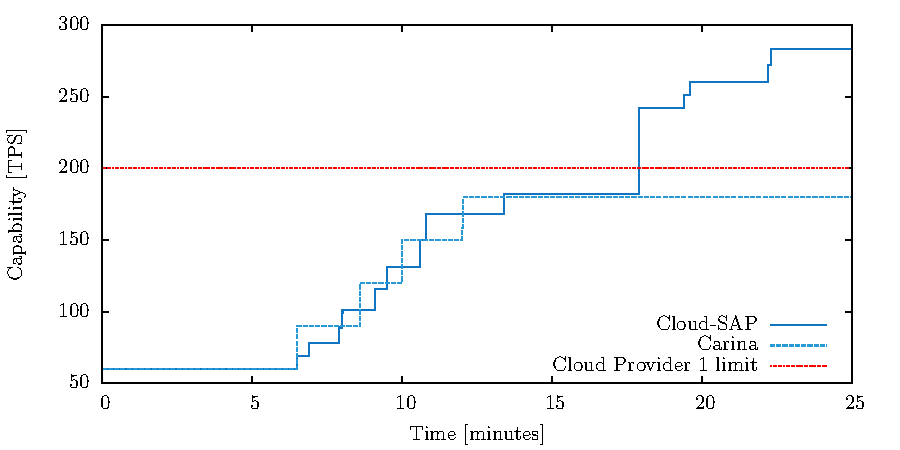
\includegraphics{chapter-evaluation/auto-scaling-2cp-tps-comparison}
  \end{center}
  \caption{Auto-scaling - multiple-provider based: comparison of processed transaction per second}
  \label{fig:auto-scaling-2cp-tps-comparison}
\end{figure}

\subsection*{Conclusion}
Comparing expectations with test output, one can see that expectations has been fully met. While \emph{Carina} was solely focused on horizontal scaling and bound to a single cloud provider, \emph{Cloud-SAP} first took fine-grained actions to later leverage resources of a second cloud provider.

\emph{Cloud-SAP} has been proven to be a better solution, offering greater capabilities to a service. This was possible by exploiting resources of two federated cloud providers, crucial concept behind \emph{Cloud-SAP} design.


\section{Deployment time -- solution comparison}
\subsection*{Description}
In this test we want to compare our solution to one of those available at the market which use \emph{OpenNebula} as an underlying tool for managing resources of a data center and \emph{OpenVZ} as a hypervisor in terms of \textbf{deployment time}, one of the most important factors of products whose main purpose is to scale applications.
\emph{Carina} \cite{Carina} can be considered a perfect match of a solution for such a comparison and tests are ran against it.

This test involves the steps of
  \begin{inparaenum}[i)]
    \item instantiating one of the tested product, i.e. Cloud-SAP or Carina,
    \item ordering the deployment of a service whose specification is shown in listing \ref{lst:service-spec-test-deployment-time},
    \item measuring the time needed to set up the environment of the service.
  \end{inparaenum}

\subsection*{Preconditions}
It is assumed that \emph{Cloud-SAP} and \emph{Carina} according with \emph{OpenVZ} as an underlying virtualization technology are correctly installed and configured.
Each test case must be run in an isolation so before performing any test all virtual machines present at the deployment node are removed.
\subsubsection{OpenNebula configuration}
To ensure objectivity in tests, OpenNebula was configured in both products in the same way. One of the key factors that could influence the deployment time is the configuration of scheduler. Its parameters are shown in the listing \ref{lst:one-scheduler-config}.
\lstinputlisting[caption=OpenNebula scheduler configuration, label=lst:one-scheduler-config]{deployment-time-test-sched-config}
\subsubsection{Service description}
The service comprises a simple java enterprise application, deployed in a master-slave configuration with one VM set as a load balancer and other nodes that serve as workers, which uses Tomcat as a web container.

The description of a service expressed in Carina format can be found in listing \ref{lst:carina-config}.

\subsubsection{Hardware configuration}

All virtual machines were deployed on a host named \emph{Node1}, whose configuration can be found in table \ref{tab:test-deployment-time-common-hardware-configuration}. Diagram presents the physical configuration of nodes.

\begin{figure}[!ht]
  \begin{center}
    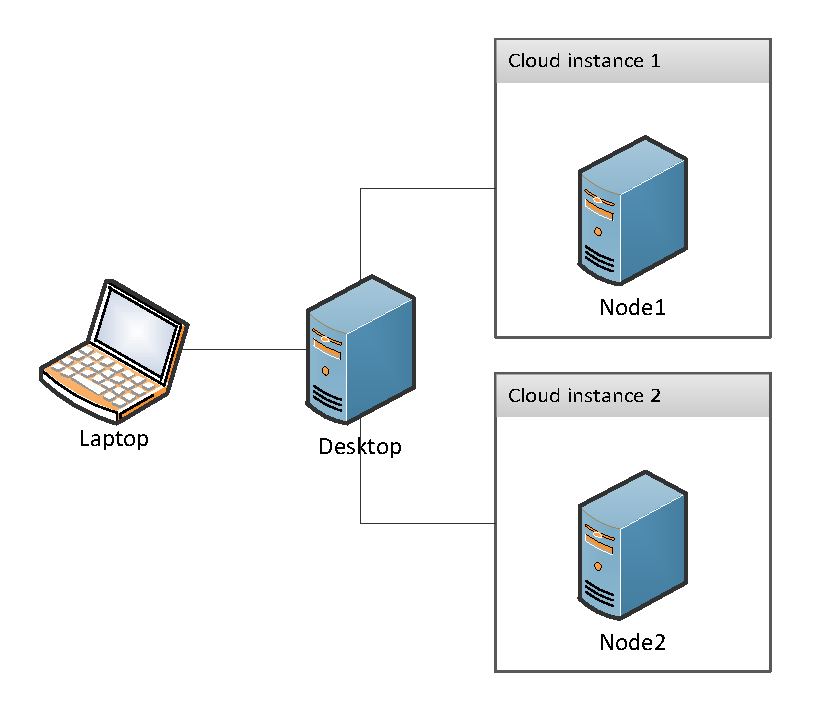
\includegraphics[width=0.6\textwidth]{chapter-evaluation/deployment-time-physical-nodes}
  \end{center}
  \caption{Deployment time - solution comparison: physical environment setup}
  \label{fig:deployment-time-physical-nodes}
\end{figure}

\newpage
\subsubsection{Environment configuration}
Deployment diagram for \emph{Carina} implementation is shown in figure \ref{ch7:deployment-time-test-deployment-time-carina-deployment-diagram} and for \emph{Cloud-SAP} in figure \ref{ch7:deployment-time-test-cloud-sap-deployment-diagram}.

\begin{figure}[!ht]
  \begin{center}
    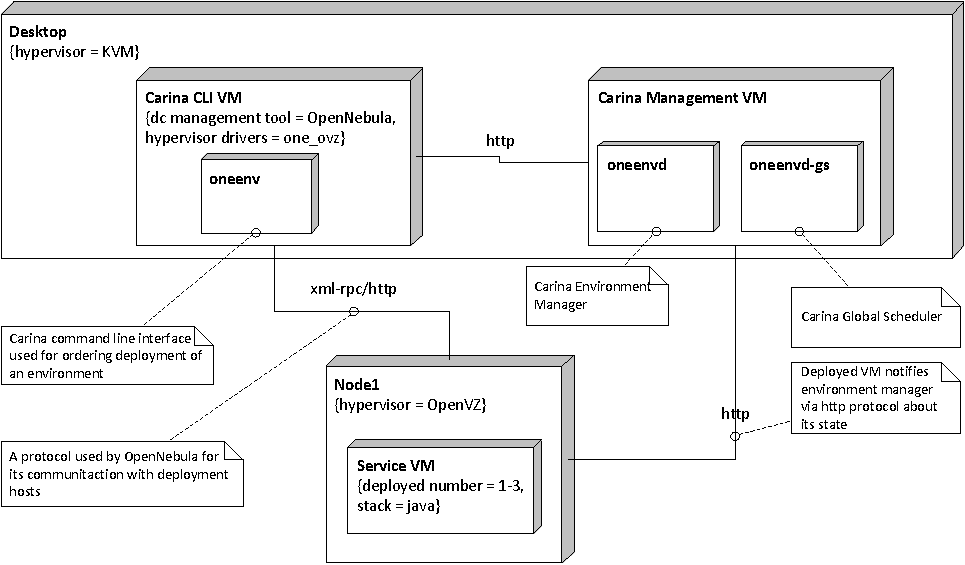
\includegraphics{chapter-evaluation/deployment-time-carina-deployment-diagram}
  \end{center}
  \caption{Deployment diagram of \emph{Carina}}
  \label{ch7:deployment-time-test-deployment-time-carina-deployment-diagram}
\end{figure}

\begin{figure}[!ht]
  \begin{center}
    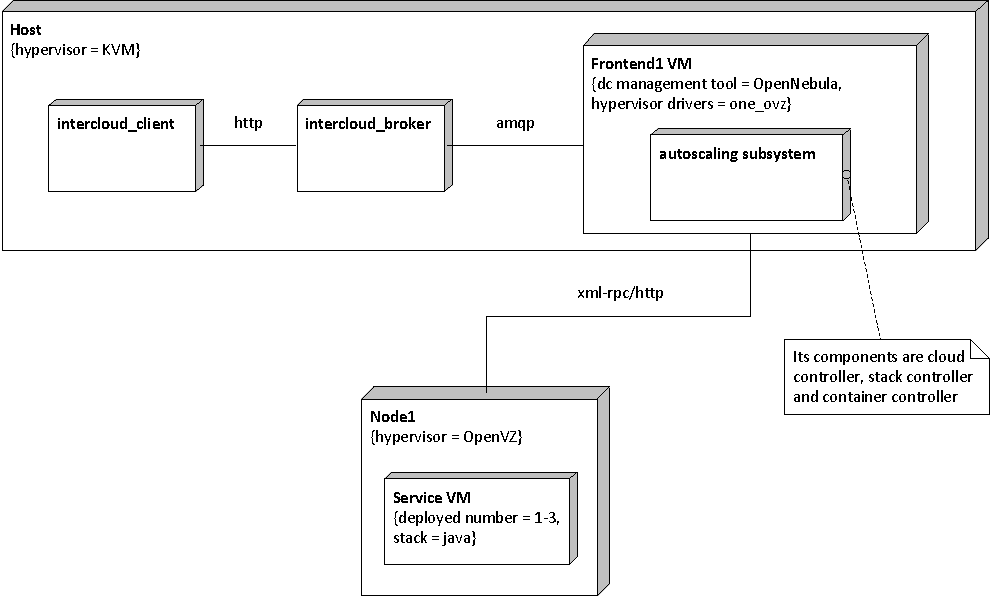
\includegraphics{chapter-evaluation/deployment-time-test-cloud-sap-deployment-diagram}
  \end{center}
  \caption{Deployment diagram of \emph{Cloud-SAP}}
  \label{ch7:deployment-time-test-cloud-sap-deployment-diagram}
\end{figure}

\newpage
\subsection*{Results}
Obtained results are shown in table \ref{tab:test-service-deployment-time} and in figure \ref{ch7:deployment-time-test}. For a given number of instances we ordered deploying a service 10 times and the values shown in those figures are an average of these runs.

\begin{table}
  \centering
  \begin{tabular}{ c  c  c }
    \specialrule{.1em}{.05em}{.05em} 
    & \multicolumn{2}{c}{\textbf{Solution}} \\
    \cline{2-3}
    \textbf{Instance no} & Cloud-SAP & Carina \\
    \specialrule{.1em}{.05em}{.05em} 
    2 & 198.0 & 158.7 \\ \hline
    3 & 261.72 & 208.1 \\ \hline
    4 & 294.38 & 230.6 \\
    \hline
  \end{tabular}
  \caption{Average deployment time for the service with the various number of VMs used for the whole environment}
  \label{tab:test-service-deployment-time}
\end{table}

\begin{figure}[!ht]
  \begin{center}
    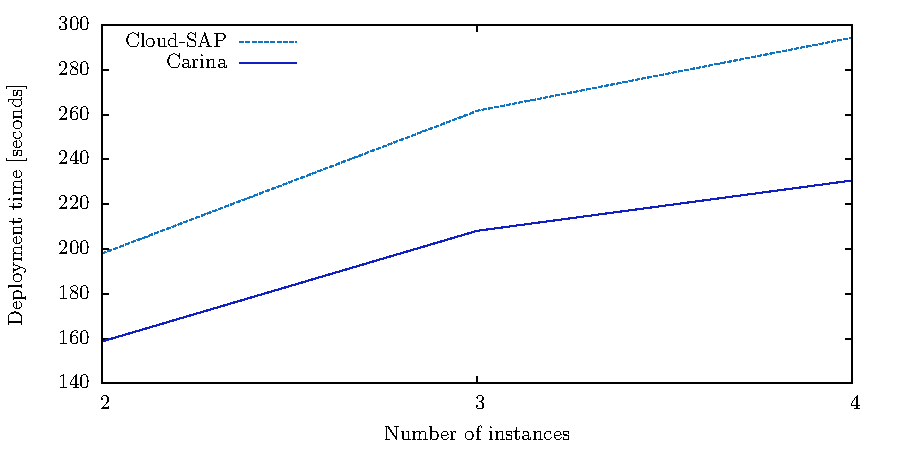
\includegraphics{chapter-evaluation/deployment-time-test}
  \end{center}
  \caption{Average deployment time for two competing products when the variable is the number of instances of VMs}
  \label{ch7:deployment-time-test}
\end{figure}

\subsection*{Conclusion}
As one can can notice, deployment of a java stack using \emph{Cloud-SAP} lasts longer than when using \emph{Carina} for the same purpose. Moreover, the more instances are in such stack, the greater difference is. This difference in provisioning time is mainly driven by the fact that \emph{Cloud-SAP} uses a great deal of components in comparison to \emph{Carina}, what is a direct consequence of chosen architecture. Specifically, the request from a client is passed to a broker, then the best provider is chosen and finally the deployment using the select provider and its \emph{Applfow} server takes place. Contrary, \emph{Carina} directly operates on \emph{OpenNebula} giving much simpler flow.

Noticeably, deployment time never was a crucial issue for \emph{Cloud-SAP}, hence, this matter is of a little importance. What is actually important for \emph{Cloud-SAP} is deployment cost and service performance. In other words, slightly greater deployment time is a price that is paid to be sure that resources are deployed optimally and with Quality-of-Service guarantee.

\chapter{Summary}

\chapterintro{This chapter provides the summary of the dissertation and gives information about future work and research directions.}

\section{Conclusions}
In this dissertation we proposed an architecture of a platform that ensures satisfying Quality of Service requirements of users' applications deployed in a cloud computing environment. The key attribute of the proposed system is holistic approach to a self-adaptability achieved by an insightful understanding of a platform-as-a-service model. As a consequence, designed architecture manages variety of resources that users' applications incorporate leading to a system that is capable of vertical, horizontal and most importantly cloud-federation aware scaling. Additionally, we implemented a minimal viable product which conforms to the devised architecture and made its evaluation by performing tests which compare it to some of the currently available solutions.

The architecture proposal and its implementation clearly indicates that the goals of the dissertation stated in the first chapter have been achieved. Since the implementation is merely a proof-of-concept, it cannot be seen as a complete or reference solution, though. Irrespective of the simplicity of the employed prediction, planning or resource mapping algorithms, promising test results were obtained. However, in order to get better results, more sophisticated algorithms and methods should be implemented in place of them.

All tests of the platform were not simulated on any software, but conducted on the real hardware forming a home-made data center. Tests were chosen so as to reflect at the highest possible rate real business use cases. Their results show considerable potential of the proposed solution. Nevertheless, we did not manage to evaluate implementation in a real-world scenario that entails using enterprise-level application such as the ones based on Java Enterprise Edition.

\section{Future work}
As the provided implementation cannot be regarded as a fully fledged one, there is a need to implement a system with the advanced algorithms regarding actions in a control loop of autonomic managers such as:
\begin{inparaenum}[1)]
  \item prediction
  \item service prioritization
  \item application self-tuning
\end{inparaenum}
This will enable to conduct more insightful tests of the architecture and prove its usefulness.

Beside this, the implementation should became a business-ready product instead of being simply a proof-of-concept. What should be done to enact it is to:
\begin{itemize}
 \item enrich Cloud-SAP architecture with a number of financial aspects such as service maintenance cost, policy and customer oriented billings (i.e. fee should take into account customer-specified policy or customer himself).
 \item evaluate solution against real-world benchmarks such as SPECweb96, SPECweb99 or TPC-C
\end{itemize}
Due to Cloud-SAP flexibility, above-mentioned features should be easily and seamlessly incorporated in proposed model.


Having more mature platform implemented and tested, next step should be to engage communities working on Open Source cloud platform such as OpenNebula, OpenStack or Eucalyptus. It is expected that such cooperation broaden pool of supported cloud providers and thus truly enable diversified federation of clouds. However, for cloud providers to cooperate, there is a need for discussion and consideration regarding aspects such as authentication, authorization, resource
 access, resource discovery, to name a few.




\appendix
\chapter{Code listings}

\section{Service specifications}
\lstinputlisting[caption=Carina Environment Specification which was used during tests of deployment time, label=lst:carina-config]{appendices/carina-svc-config.rb}

\lstinputlisting[caption=Cloud-SAP Service Specification (without scaling policies), label=lst:service-spec-test-cost]{appendices/service-spec-test-cost.json}

\lstinputlisting[caption=Cloud-SAP Service Specification used for testing deployment time, label=lst:service-spec-test-deployment-time]{appendices/service-spec-deployment-time-test.json}

\section{Scaling policies}
\label{app:scaling-policies}

Listings \ref{lst:scaling-ec2} illustrates XML-based policy that is used by Auto Scaling of the Amazon Web Services EC2.
\lstinputlisting[caption=Scaling policy - AWS EC2, label=lst:scaling-ec2]{appendices/scaling-policy.xml}



\listoftables
\clearpage
\listoffigures

\bibliographystyle{acm}
\bibliography{thesis}

\end{document}
